\documentclass[10pt,aspectratio=169]{beamer}
% \documentclass[10pt,aspectratio=169,handout]{beamer}

% silence some Metropolis warnings
\usepackage{silence}
\WarningFilter{beamerthememetropolis}{You need to compile with XeLaTeX or LuaLaTeX}
\WarningFilter{latexfont}{Font shape}
\WarningFilter{latexfont}{Some font}

% define custom colors
\definecolor{dark gray}{HTML}{444444}
\definecolor{light gray}{HTML}{777777}
\definecolor{dark red}{HTML}{BB0000}
\definecolor{dark green}{HTML}{00BB00}

% configure metropolis
\usetheme[numbering=fraction]{metropolis}
\setbeamercolor{background canvas}{bg=white}
\setbeamercolor{frametitle}{bg=dark gray}
\setbeamercolor{alerted text}{fg=dark red}
\setbeamercolor{item projected}{bg=dark red}
\setbeamercolor{local structure}{fg=dark red}
\setbeamersize{text margin left=0.5cm,text margin right=0.5cm}
\setbeamercovered{transparent=10}

% use thicker lines
\makeatletter
\setlength{\metropolis@titleseparator@linewidth}{1pt}
\setlength{\metropolis@progressonsectionpage@linewidth}{1pt}
\makeatother

% custom bullet points
\setbeamertemplate{itemize item}{\color{dark red}$\blacktriangleright$}
\setbeamertemplate{itemize subitem}{\color{dark red}$\blacktriangleright$}
\setbeamertemplate{itemize subsubitem}{\color{dark red}$\blacktriangleright$}
\newcommand{\custombullet}{{\color{dark red}$\blacktriangleright$}\hspace{0.5em}}

% use classic font for math
\usefonttheme[onlymath]{serif}

% imports
\usepackage[english]{babel}
\usepackage[utf8]{inputenc}
\usepackage{amsthm}
\usepackage{amssymb}
\usepackage{amsmath}
\usepackage{amsfonts}
\usepackage{mathtools}
\usepackage{mathabx}
\usepackage{stmaryrd}
\usepackage{graphicx}
\usepackage{hyperref}
\usepackage{xfrac}
\usepackage{appendixnumberbeamer}

% check and x marks
\usepackage{pifont}
\newcommand{\cmark}{{\color{dark green}\ding{51}}\hspace{0.3em}}
\newcommand{\xmark}{{\color{dark red}\ding{55}}\hspace{0.5em}}

% diagrams
\usepackage{tikz}
\usetikzlibrary{decorations.pathreplacing}

% references
\usepackage[natbibapa]{apacite}
\bibliographystyle{apacite}
\renewcommand{\bibsection}{}

% use ampersands instead of "and" for text citations
\AtBeginDocument{\renewcommand{\BBAB}{\&}}

% possessive cites
\makeatletter
\patchcmd{\NAT@test}{\else \NAT@nm}{\else \NAT@nmfmt{\NAT@nm}}{}{}
\DeclareRobustCommand\citepos
  {\begingroup
   \let\NAT@nmfmt\NAT@posfmt
   \NAT@swafalse\let\NAT@ctype\z@\NAT@partrue
   \@ifstar{\NAT@fulltrue\NAT@citetp}{\NAT@fullfalse\NAT@citetp}}
\let\NAT@orig@nmfmt\NAT@nmfmt
\def\NAT@posfmt#1{\NAT@orig@nmfmt{#1's}}
\makeatother

% spaced-out lists
\newenvironment{wideitemize}{\itemize\addtolength{\itemsep}{10pt}}{\enditemize}
\newenvironment{wideenumerate}{\enumerate\addtolength{\itemsep}{10pt}}{\endenumerate}

% replace footnotes with buttons
\usepackage[absolute,overlay]{textpos}
\newcounter{beamerpausessave}
\newcommand{\always}[1]{
    \setcounter{beamerpausessave}{\value{beamerpauses}}
    \setcounter{beamerpauses}{0}
    \pause
    #1 
    \setcounter{beamerpauses}{\value{beamerpausessave}}
    \addtocounter{beamerpauses}{-1}
    \pause
}
\newcommand{\buttons}[1]{\always{
    \begin{textblock*}{\paperwidth}(0.015\textwidth, 1.022\textheight)
        \scriptsize
        #1
    \end{textblock*}
}}
\newcommand{\appendixbuttons}[1]{\always{
    \begin{textblock*}{\paperwidth}(0.015\textwidth, 1.043\textheight)
        \scriptsize
        #1
    \end{textblock*}
}}
\newcommand{\goto}[2]{\hyperlink{#1}{{\color{dark red}$\smalltriangleright$} #2}\hspace{0.5em}}
\newcommand{\goback}[2]{\hyperlink{#1}{{\color{dark red}$\smalltriangleleft$} #2}\hspace{0.5em}}

% custom appendix
\renewcommand{\appendixname}{\texorpdfstring{\translate{Appendix}}{Appendix}}

% change color of cites and URLs
\let\oldcite\cite
\let\oldcitet\citet
\let\oldcitep\citep
\let\oldcitepos\citepos
\let\oldcitetalias\citetalias
\let\oldcitepalias\citepalias
\let\oldurl\url
\def\cite#1#{\citeaux{#1}}
\def\citet#1#{\citetaux{#1}}
\def\citep#1#{\citepaux{#1}}
\def\citepos#1#{\citeposaux{#1}}
\def\citetalias#1#{\citetaliasaux{#1}}
\def\citepalias#1#{\citepaliasaux{#1}}
\def\url#1#{\urlaux{#1}}
\newcommand*\citeaux[2]{{\color{light gray}\oldcite#1{#2}}}
\newcommand*\citetaux[2]{{\color{light gray}\oldcitet#1{#2}}}
\newcommand*\citepaux[2]{{\color{light gray}\oldcitep#1{#2}}}
\newcommand*\urlaux[2]{{\color{light gray}\oldurl#1{#2}}}
\newcommand*\citeposaux[2]{{\color{light gray}\oldcitepos#1{#2}}}
\newcommand*\citetaliasaux[2]{{\color{light gray}\oldcitetalias#1{#2}}}
\newcommand*\citepaliasaux[2]{{\color{light gray}\oldcitepalias#1{#2}}}

% custom math commands
\DeclareMathOperator*{\argmax}{argmax}
\DeclareMathOperator*{\argmin}{argmin}
\renewcommand{\Pr}{\mathbb{P}}
\newcommand{\E}{\mathbb{E}}
\newcommand{\Var}{\mathbb{V}}
\newcommand{\Cov}{\mathbb{C}}
\newcommand{\overbar}[1]{\mkern 1.5mu\overline{\mkern-1.5mu#1\mkern-1.5mu}\mkern 1.5mu}

% tables
\usepackage{booktabs}
\usepackage{colortbl}
\usepackage{multirow}
\usepackage{makecell}
\arrayrulecolor{dark red}

% custom date
\usepackage{datetime}
\newdateformat{monthyeardate}{\monthname[\THEMONTH] \THEYEAR}

% fix pauses with graphics
\usepackage{fixpauseincludegraphics}


\usepackage{lipsum}
\usepackage{amsmath} 
\usepackage{amsthm} 
\usepackage{amssymb} 
\usepackage{mathtools}
%\usepackage{natbib}
\usepackage{dutchcal}


\newcommand{\vect}[1]{\boldsymbol{\mathbf{#1}}}
\newcommand{\pd}[2]{\frac{\partial{#1}}{\partial{#2}}}
\newcommand{\expect}[2]{\mathbb{E}_{#1}\left[{#2}\right]}
\newcommand{\expectsmall}[2]{\mathbb{E}_{#1}{#2}}
\newcommand{\expectsuper}[3]{\mathbb{E}_{#1}^{#2}\left[{#3}\right]}
\newcommand{\ind}[1]{\mathbbm{1}\left\{{#1}\right\}}
\newcommand{\prob}[1]{\mathbb{P}\left\{{#1}\right\}}
\newcommand{\derivative}[2]{\frac{d{#2}}{d{#1}}}
\newcommand{\cat}[1]{\citeasnoun{#1}}

% title page
\title{Case Studies}
\author{Chris Conlon}
\institute{NYU Stern and NBER}

\date{Summer 2023}




\begin{document}



%--------------
% TITLE PAGE
\begin{frame}[plain] %
\titlepage
\end{frame}



\section*{Conlon and Rao (2014/2023) on Distilled Spirits}



\begin{frame}{Why does supply matter? (Conlon Rao 2014/2023)}
\begin{itemize}
\item Looked at a wholesale price posting law challenged under the Sherman Act
\begin{itemize}
\item Post your prices
\item Look at competitors prices
\item Can meet but not beat them.
\item \textrightarrow Everyone sets monopoly price and then matches
\end{itemize}
\item We can calculate $\eta_{jt}$ markups using game theory
\item We observe $\mathbf{p^w}$ (wholesale) and $\mathbf{p^m}$ (manufacturer) and $\tau_{jt}$ (taxes).
\begin{itemize}
\item We basically know $MC$!
\end{itemize}
\end{itemize}
\end{frame}






\begin{frame}{Why does supply matter? (Conlon Rao 2014/2023)}
Consumer $i$ chooses product $j$ (brand-size-flavor) in quarter $t$:
\begin{align*}
u_{ijt} &= \beta_{i}^0 -  \alpha_i\, p_{jt} + \beta_i^{1750}\, \cdot \mathbb{I}[1750mL]_j + \gamma_j + \gamma_t+ \varepsilon_{ijt}(\rho)\\
\begin{pmatrix}
\ln \alpha_i\\
\beta_i
\end{pmatrix} &=
\begin{pmatrix}
\overline{\alpha}\\
\theta_1
\end{pmatrix} + \Sigma \cdot \nu_i + \sum_{k} \Pi_k \cdot \mathbb{I}\{LB_k \leq \text{Income}_i < UB_k\} 
\end{align*}
\begin{itemize}
\item Nesting Parameter $\rho$: Substitution within category (Vodka, Gin, etc.) %(Vodka/Tequila/Rum/Gin/Whiskey)
\item Consumers of different income levels have different mean values for coefficients
\item Conditional on income, normally distributed unobserved heterogeneity for:
\begin{itemize}
\item Price $\alpha_i$
\item Constant $\beta_{i}^0$ (Overall demand for spirits)
\item Package Size: $\beta_{i}^{1750}$ (Large vs. small bottles)
\end{itemize}
\end{itemize}
\end{frame}


\begin{frame}{Wholesale Margins Under Post and Hold}
\begin{columns}[T]
\begin{column}{.5\textwidth}
\begin{center}
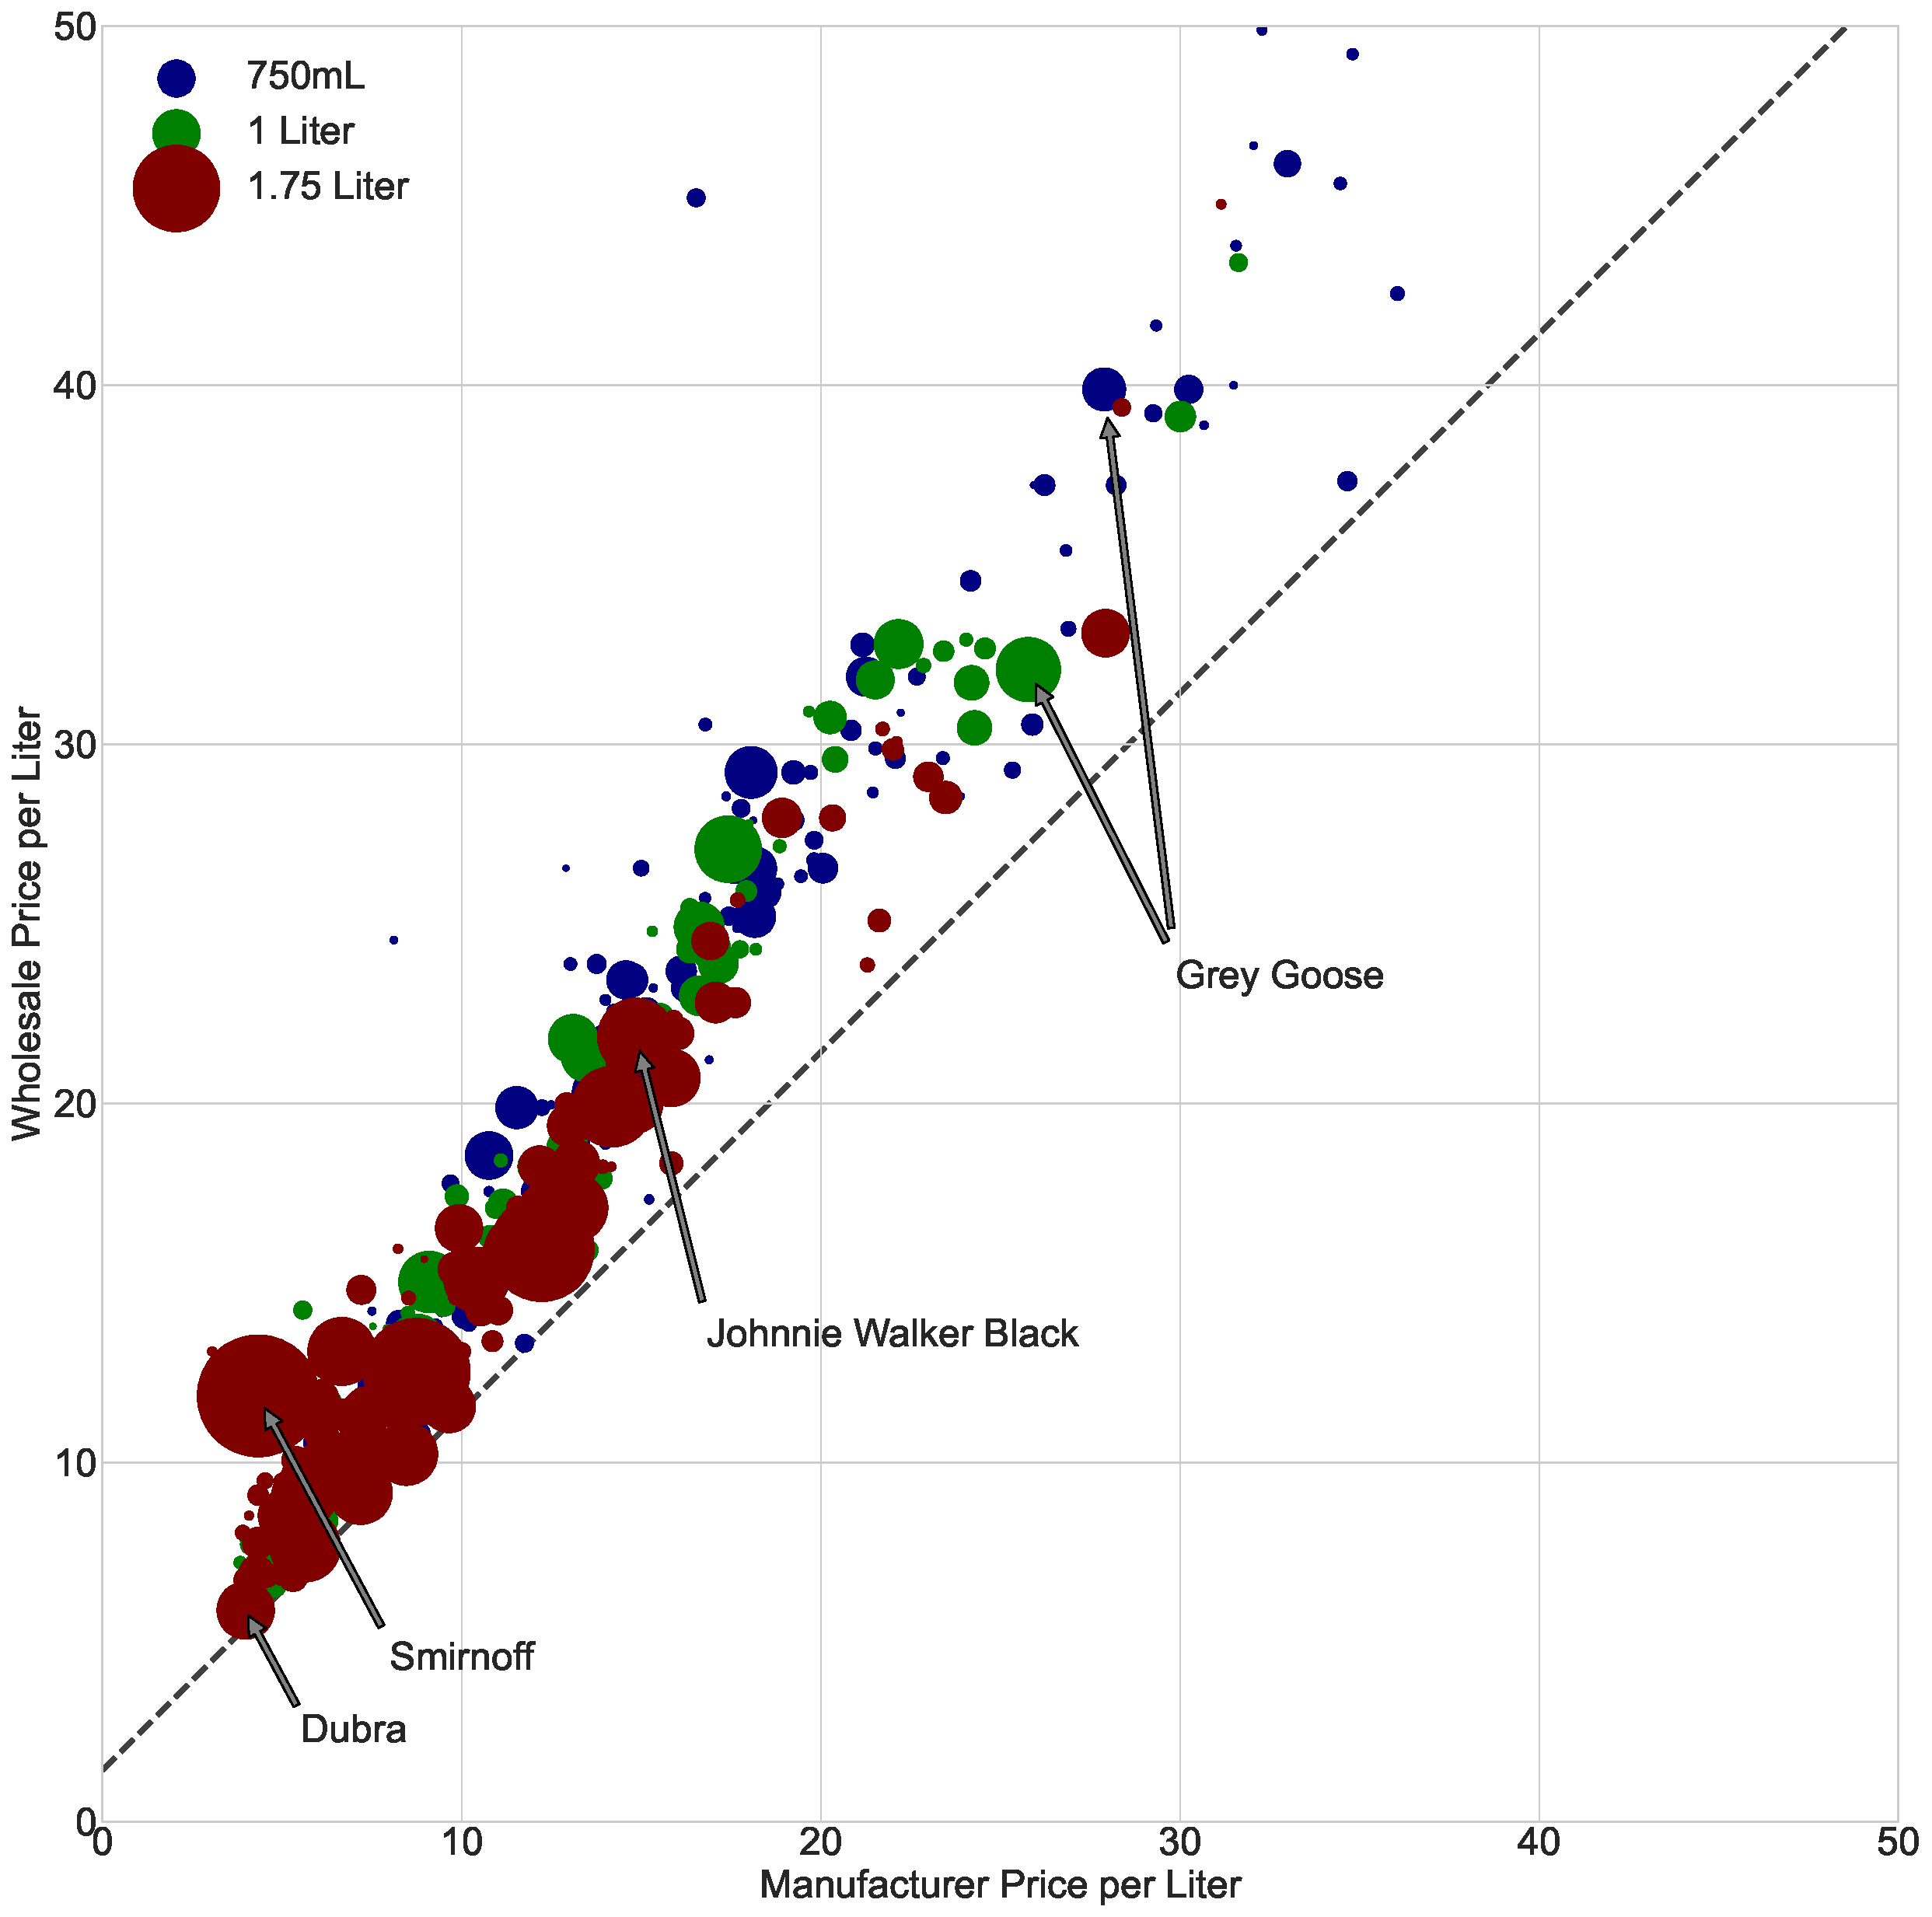
\includegraphics[height=0.88\textheight]{../demand/resources/figure4_manuf_wholesale_price.pdf}
\end{center}
\end{column}
\hfill
\begin{column}{.5\textwidth}
  \begin{itemize}
  \item Price Cost Margins (and Lerner Markups) are higher on premium products
  \item Markups on least expensive products (plastic bottle vodka) are very low.
  \item Smirnoff (1.75L) is best seller\\ (high markup / outlier).
  \item A planner seeking to minimize ethanol consumption would flatten these markups!
  \item Matching this pattern is kind of the whole ballgame !
  \item Plain logit gives $\epsilon_{jj} = \alpha \cdot p_j  \cdot (1-s_j)$.
  \end{itemize}
  \end{column}
\end{columns}
\end{frame}



\begin{frame}{Demand Estimates (from \texttt{PyBLP}, Conlon Gortmaker (2020, 2023))}
\begin{columns}[T]
 \hspace{-1.5cm}
 \begin{column}{.68\textwidth}
\vspace{-0.3cm}
    \begin{center}
    \scalebox{0.55}{
     \begin{tabular}{lccc} 
\toprule 
\multicolumn{1}{c}{$\Pi$} &  Const &  Price &  1750mL \\ 
\cmidrule(r){1-1} \cmidrule(rrr){2-4} 
Below \$25k  &  2.928 & -0.260 &   0.543 \\
            &  (0.233) &  (0.056) &   (0.075) \\
\$25k-\$45k   &  0.184 & -0.170 &   0.536 \\
            &  (0.236) &  (0.054) &   (0.083) \\
\$45k-\$70k   &  0.000 & -0.179 &   0.980 \\
            &  (0.000) &  (0.053) &   (0.093) \\
\$70k-\$100k  & -0.452 & -0.496 &   0.608 \\
            &  (0.227) &  (0.051) &   (0.079) \\
Above \$100k & -1.777 & -1.543 &   0.145 \\
            &  (0.234) &  (0.047) &   (0.055) \\
\midrule \multicolumn{1}{c}{$\Sigma^2$}& \multicolumn{2}{c}{} \\ \cmidrule(r){1-1} \cmidrule(rrr){2-4}
Price       &  0.000 &  0.697 &   0.695 \\
            &  (0.107) &  (0.028) &   (0.048) \\
1750mL      &  0.000 &  0.695 &   1.167 \\
            &  (0.086) &  (0.048) &   (0.236) \\
\midrule  
\multicolumn{1}{l}{Nesting Parameter $\rho$} &  &0.423&    \\ 
& &(0.026)&     \\ 
\multicolumn{1}{l}{Fixed Effects} &   \multicolumn{3}{c}{Brand+Quarter}\\ 
\midrule 
%\multicolumn{1}{c}{}& \multicolumn{3}{c}{Model Predictions} \\ 
\multicolumn{1}{c}{Model Predictions}& 25\% & 50\% & 75\% \\ \midrule\midrule
Own Elasticity:  $\frac{\partial \log q_j}{\partial \log p_j}$                  & -5.839 & -5.162 & -4.733 \\
Aggregate Elasticity: $\frac{\partial \log Q}{\partial \log P}$            & -0.333 & -0.329 & -0.322 \\
Own Pass-Through: $\frac{\partial p_j}{\partial c_j}$          & 1.256 & 1.284 &  1.320 \\
Observed Wholesale Markup (PH)  &  0.188 &  0.233 &  0.276 \\
Predicted Wholesale Markup (PH) &  0.205 &  0.231 &  0.259 \\
\bottomrule 
\end{tabular}
    }
    \end{center}
  \end{column}
  \hfill
 \hspace{-2.2cm}
\begin{column}{.55\textwidth}
  \begin{itemize}
    \item Demographic Interactions w/ 5 income bins \\ (matched to micro-moments)
    \item Correlated Normal Tastes: (Constant, Large Size, Price)
    \item Supply moments exploit observed upstream prices and tax change (ie: match observed markups).
    \vspace{-0.2cm}
    \begin{align*}
    \mathbb{E}[\omega_{jt}]=0, \text{ with }\omega_{jt} = \left(p^w_{jt}  - p^m_{jt}-\tau_{jt} \right) -\eta_{jt}\left(\theta_2\right).
    \end{align*}
   \vspace{-0.8cm}
    \item Match estimate of aggregate elasticity from tax change $\varepsilon=-0.4$.
    \item Pass-through consistent with estimates from our AEJ:Policy paper.
  \end{itemize}
\end{column}
\end{columns}
\end{frame}

\begin{frame}{Elasticities and Diversion Ratios}
\begin{center}
    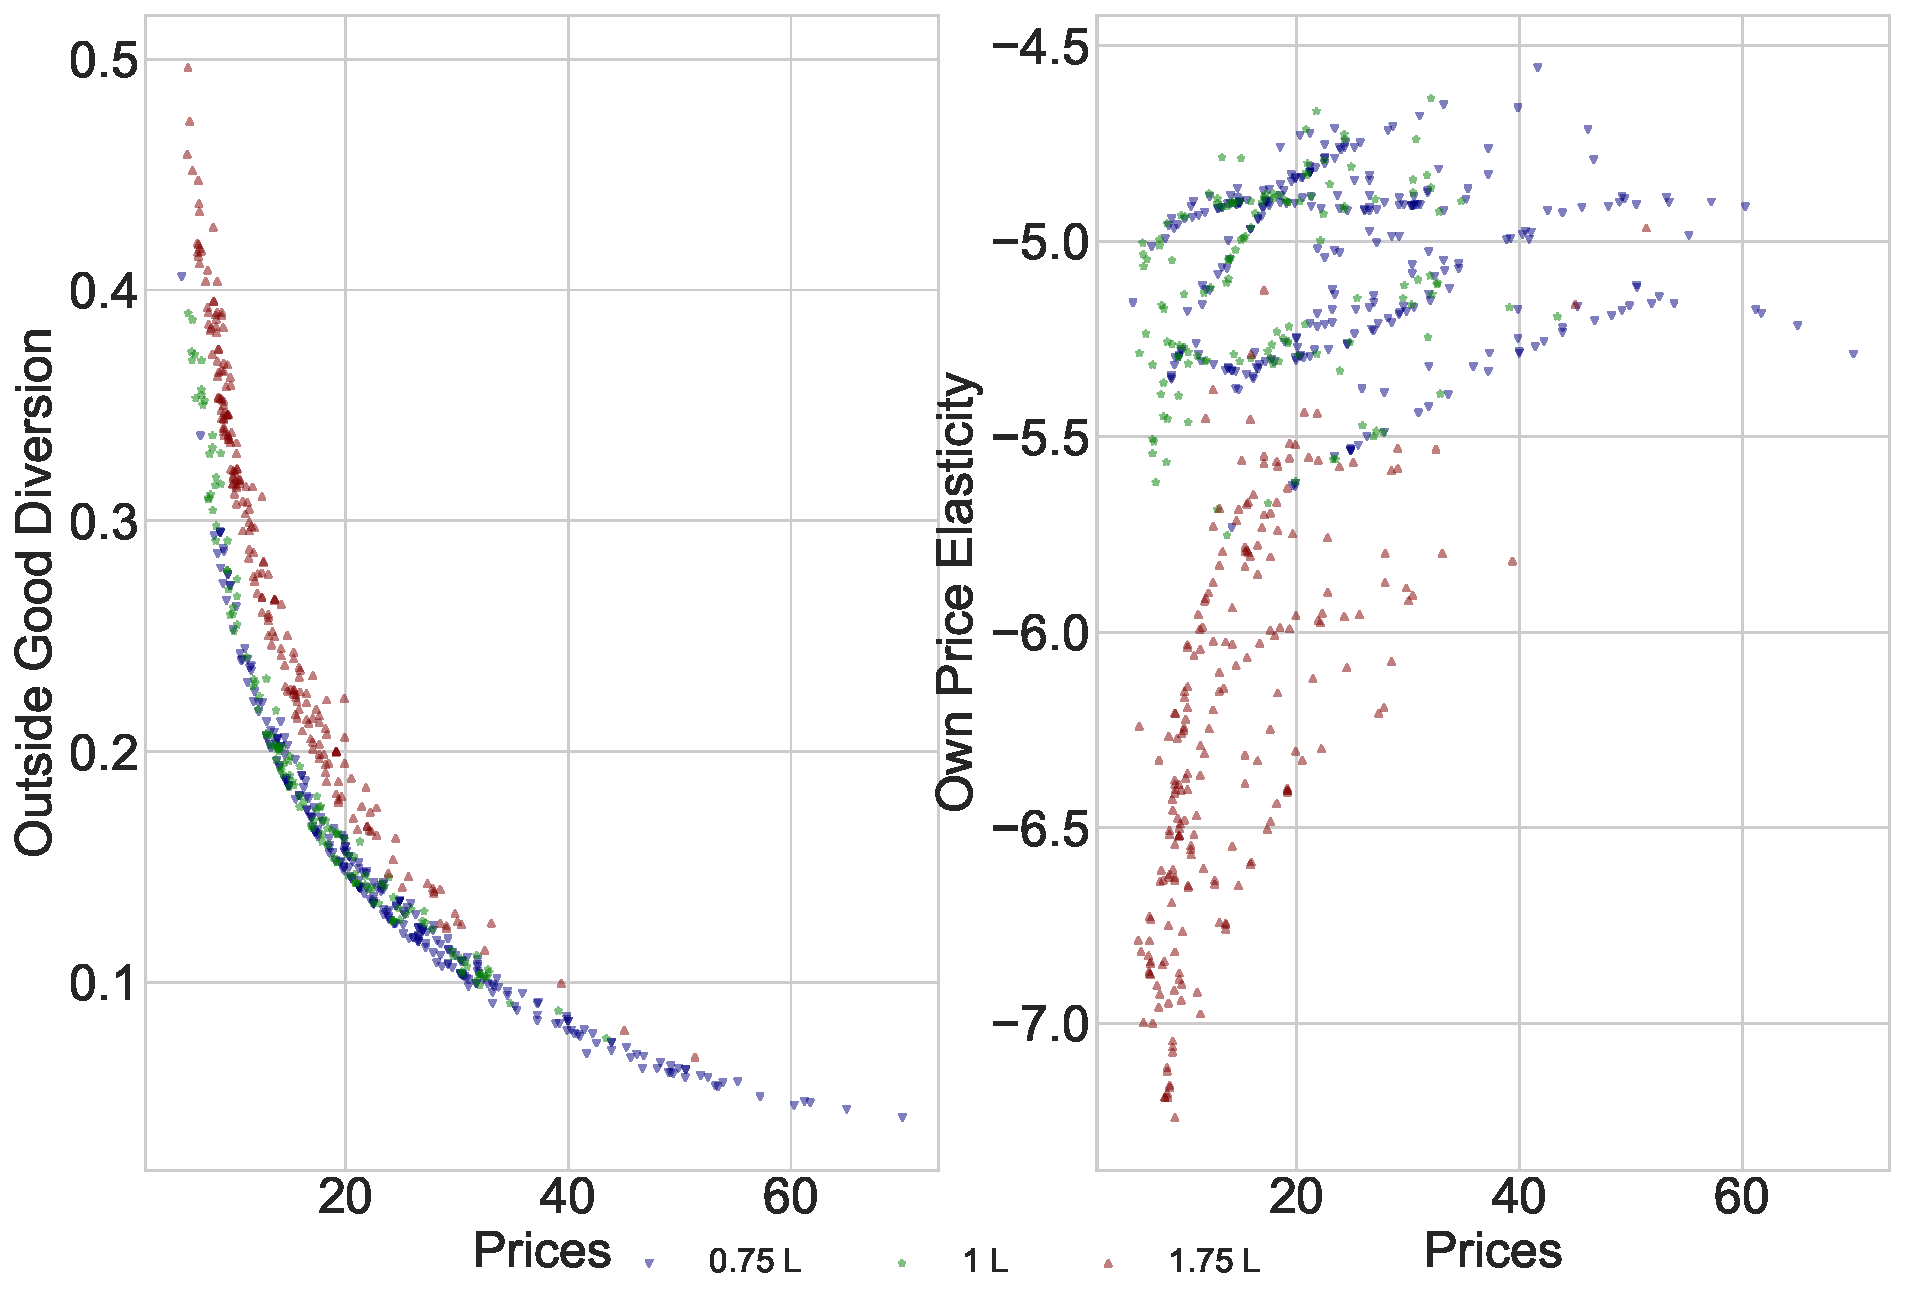
\includegraphics[height=0.95\textheight]{../demand/resources/figure6_outside_diversion_elas_v2.pdf}
\end{center}
\end{frame}



\begin{frame}{Diversion Ratios}
\begin{center}
\scalebox{0.6}{
 \begin{tabular}{lrrlrr} 
\toprule 
{}&  Median Price &  \% Substitution &  {}&  Median Price &  \% Substitution \\ 
\midrule 
\multicolumn{1}{c}{Capt Morgan Spiced 1.75 L (\$15.85)} & \multicolumn{5}{c}{ Cuervo Gold 1.75 L (\$18.33) } \\ \cmidrule(lr){1-1} \cmidrule(lrr){4-6} 
\midrule 
        Bacardi Superior Lt Dry Rum 1.75 L & 12.52 & 13.07 &                    Don Julio Silver 1.75 L & 22.81 & 5.00 \\
                   Bacardi Dark Rum 1.75 L & 12.52 &  2.71 &                          Cuervo Gold 1.0 L & 21.32 & 3.82 \\
         Bacardi Superior Lt Dry Rum 1.0 L & 15.03 &  2.44 &              Sauza Giro Tequila Gold 1.0 L &  8.83 & 3.07 \\
                           Smirnoff 1.75 L & 11.85 &  2.36 &                            Smirnoff 1.75 L & 11.85 & 2.44 \\
     Lady Bligh Spiced V Island Rum 1.75 L &  9.43 &  2.18 &                       Absolut Vodka 1.75 L & 15.94 & 2.06 \\
\midrule 
\multicolumn{1}{c}{Woodford 0.75 L (\$34.55)} & \multicolumn{5}{c}{ Beefeater Gin 1.75 L (\$17.09) } \\ \cmidrule(lr){1-1} \cmidrule(lrr){4-6} 
\midrule 
             Jack Daniel Black Label 1.0 L & 27.08 & 7.66 &                           Tanqueray 1.75 L & 17.09 & 12.80 \\
            Jack Daniel Black Label 1.75 L & 21.85 & 4.91 &                             Gordons 1.75 L & 11.19 &  4.14 \\
            Jack Daniel Black Label 0.75 L & 29.21 & 4.83 &                        Seagrams Gin 1.75 L & 10.23 &  2.85 \\
                         Makers Mark 1.0 L & 32.79 & 4.52 &                              Bombay 1.75 L & 21.95 &  2.27 \\
                        Makers Mark 0.75 L & 31.88 & 2.80 &                            Smirnoff 1.75 L & 11.85 &  2.27 \\
\midrule 
\multicolumn{1}{c}{Dubra Vdk Dom 80P 1.75 L (\$5.88)} & \multicolumn{5}{c}{ Belvedere Vodka 0.75 L (\$30.55) } \\ \cmidrule(lr){1-1} \cmidrule(lrr){4-6} 
\midrule 
                        Popov Vodka 1.75 L &  7.66 & 7.56 &                           Grey Goose 1.0 L & 32.08 & 5.09 \\
                           Smirnoff 1.75 L & 11.85 & 3.15 &                       Absolut Vodka 1.75 L & 15.94 & 3.82 \\
                    Sobieski Poland 1.75 L &  9.09 & 3.14 &                        Absolut Vodka 1.0 L & 24.91 & 2.74 \\
                 Grays Peak Vdk Dom 1.75 L &  9.16 & 2.87 &                            Smirnoff 1.75 L & 11.85 & 2.43 \\
                        Wolfschmidt 1.75 L &  6.92 & 2.48 &                          Grey Goose 0.75 L & 39.88 & 2.22 \\
\bottomrule 
\end{tabular}
}
\end{center}
\end{frame}


\section*{Backus, Conlon, Sinkinson (2021): RTE Cereal}

\begin{frame}{Implementation: Demand Specification}
\begin{gather*}
u_{ijt} =  h_d(\textrm{x}_{jt}^{(1)}, \textrm{v}_{jt}; \theta_1) - \alpha\, p_{jt} + \lambda \, \log(\text{ad}_{jt})  + \left(\Sigma \, \nu_i + \Pi\, y_i \right) \cdot x_{jt}^{(2)}+ \xi_{jt} + \varepsilon_{ijt}\\
\end{gather*}
\vspace{-0.75cm}
\begin{itemize}
\item $y_i$ demographics: estimated at the $\texttt{dma-chain-year}$ level (from panelists)
\item $y_i$ is joint distribution of $(income, kids)$
\begin{enumerate}
\item Fit a lognormal for income to households w/ and w/o kids.
\end{enumerate}
\item $\nu_i$ are random (normal) draws; price is lognormal.
\item Lots of FE in $h_d(\cdot)$ (product, chain-dma, year, week of year)
\item IV: Cost shifters, GH/Optimal IV $f(x_{-j})$, lagged advertising.
\end{itemize}
\end{frame}

\begin{frame}[plain]
\begin{center}
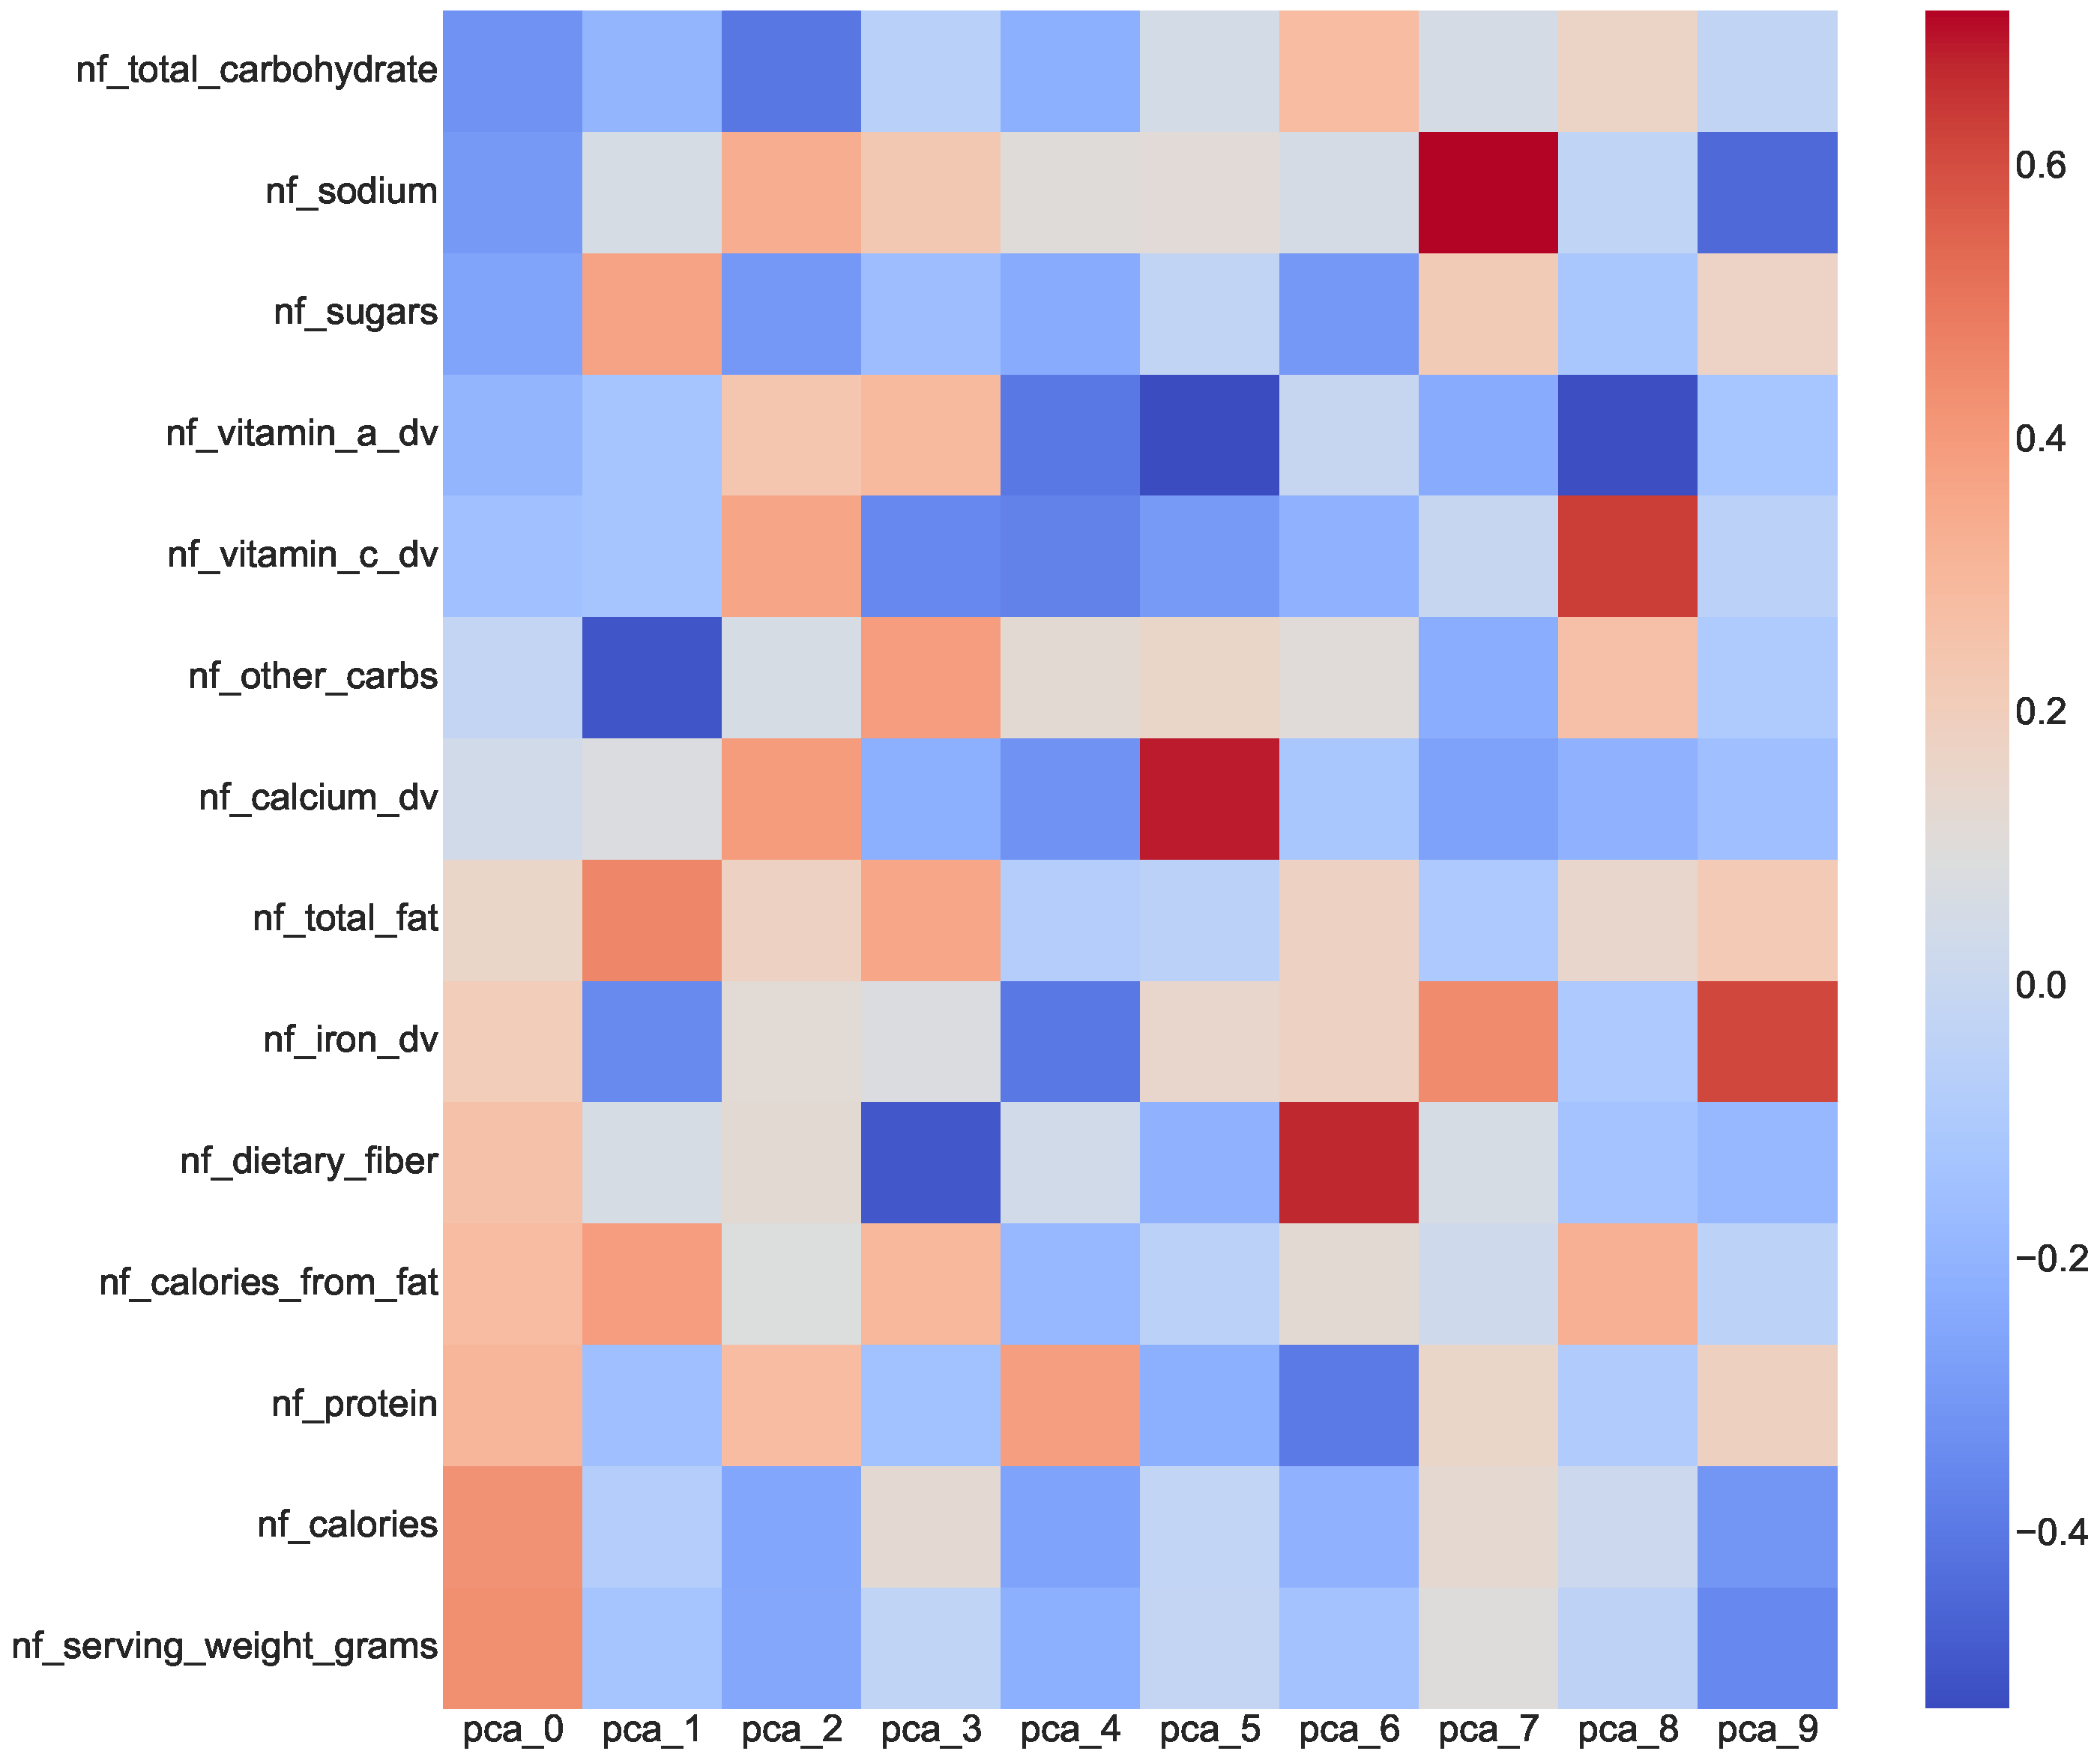
\includegraphics[height = \textheight ]{../common ownership/figures/pca_coeff.pdf}
\end{center}
\end{frame}


\begin{frame}[plain]
\begin{center}
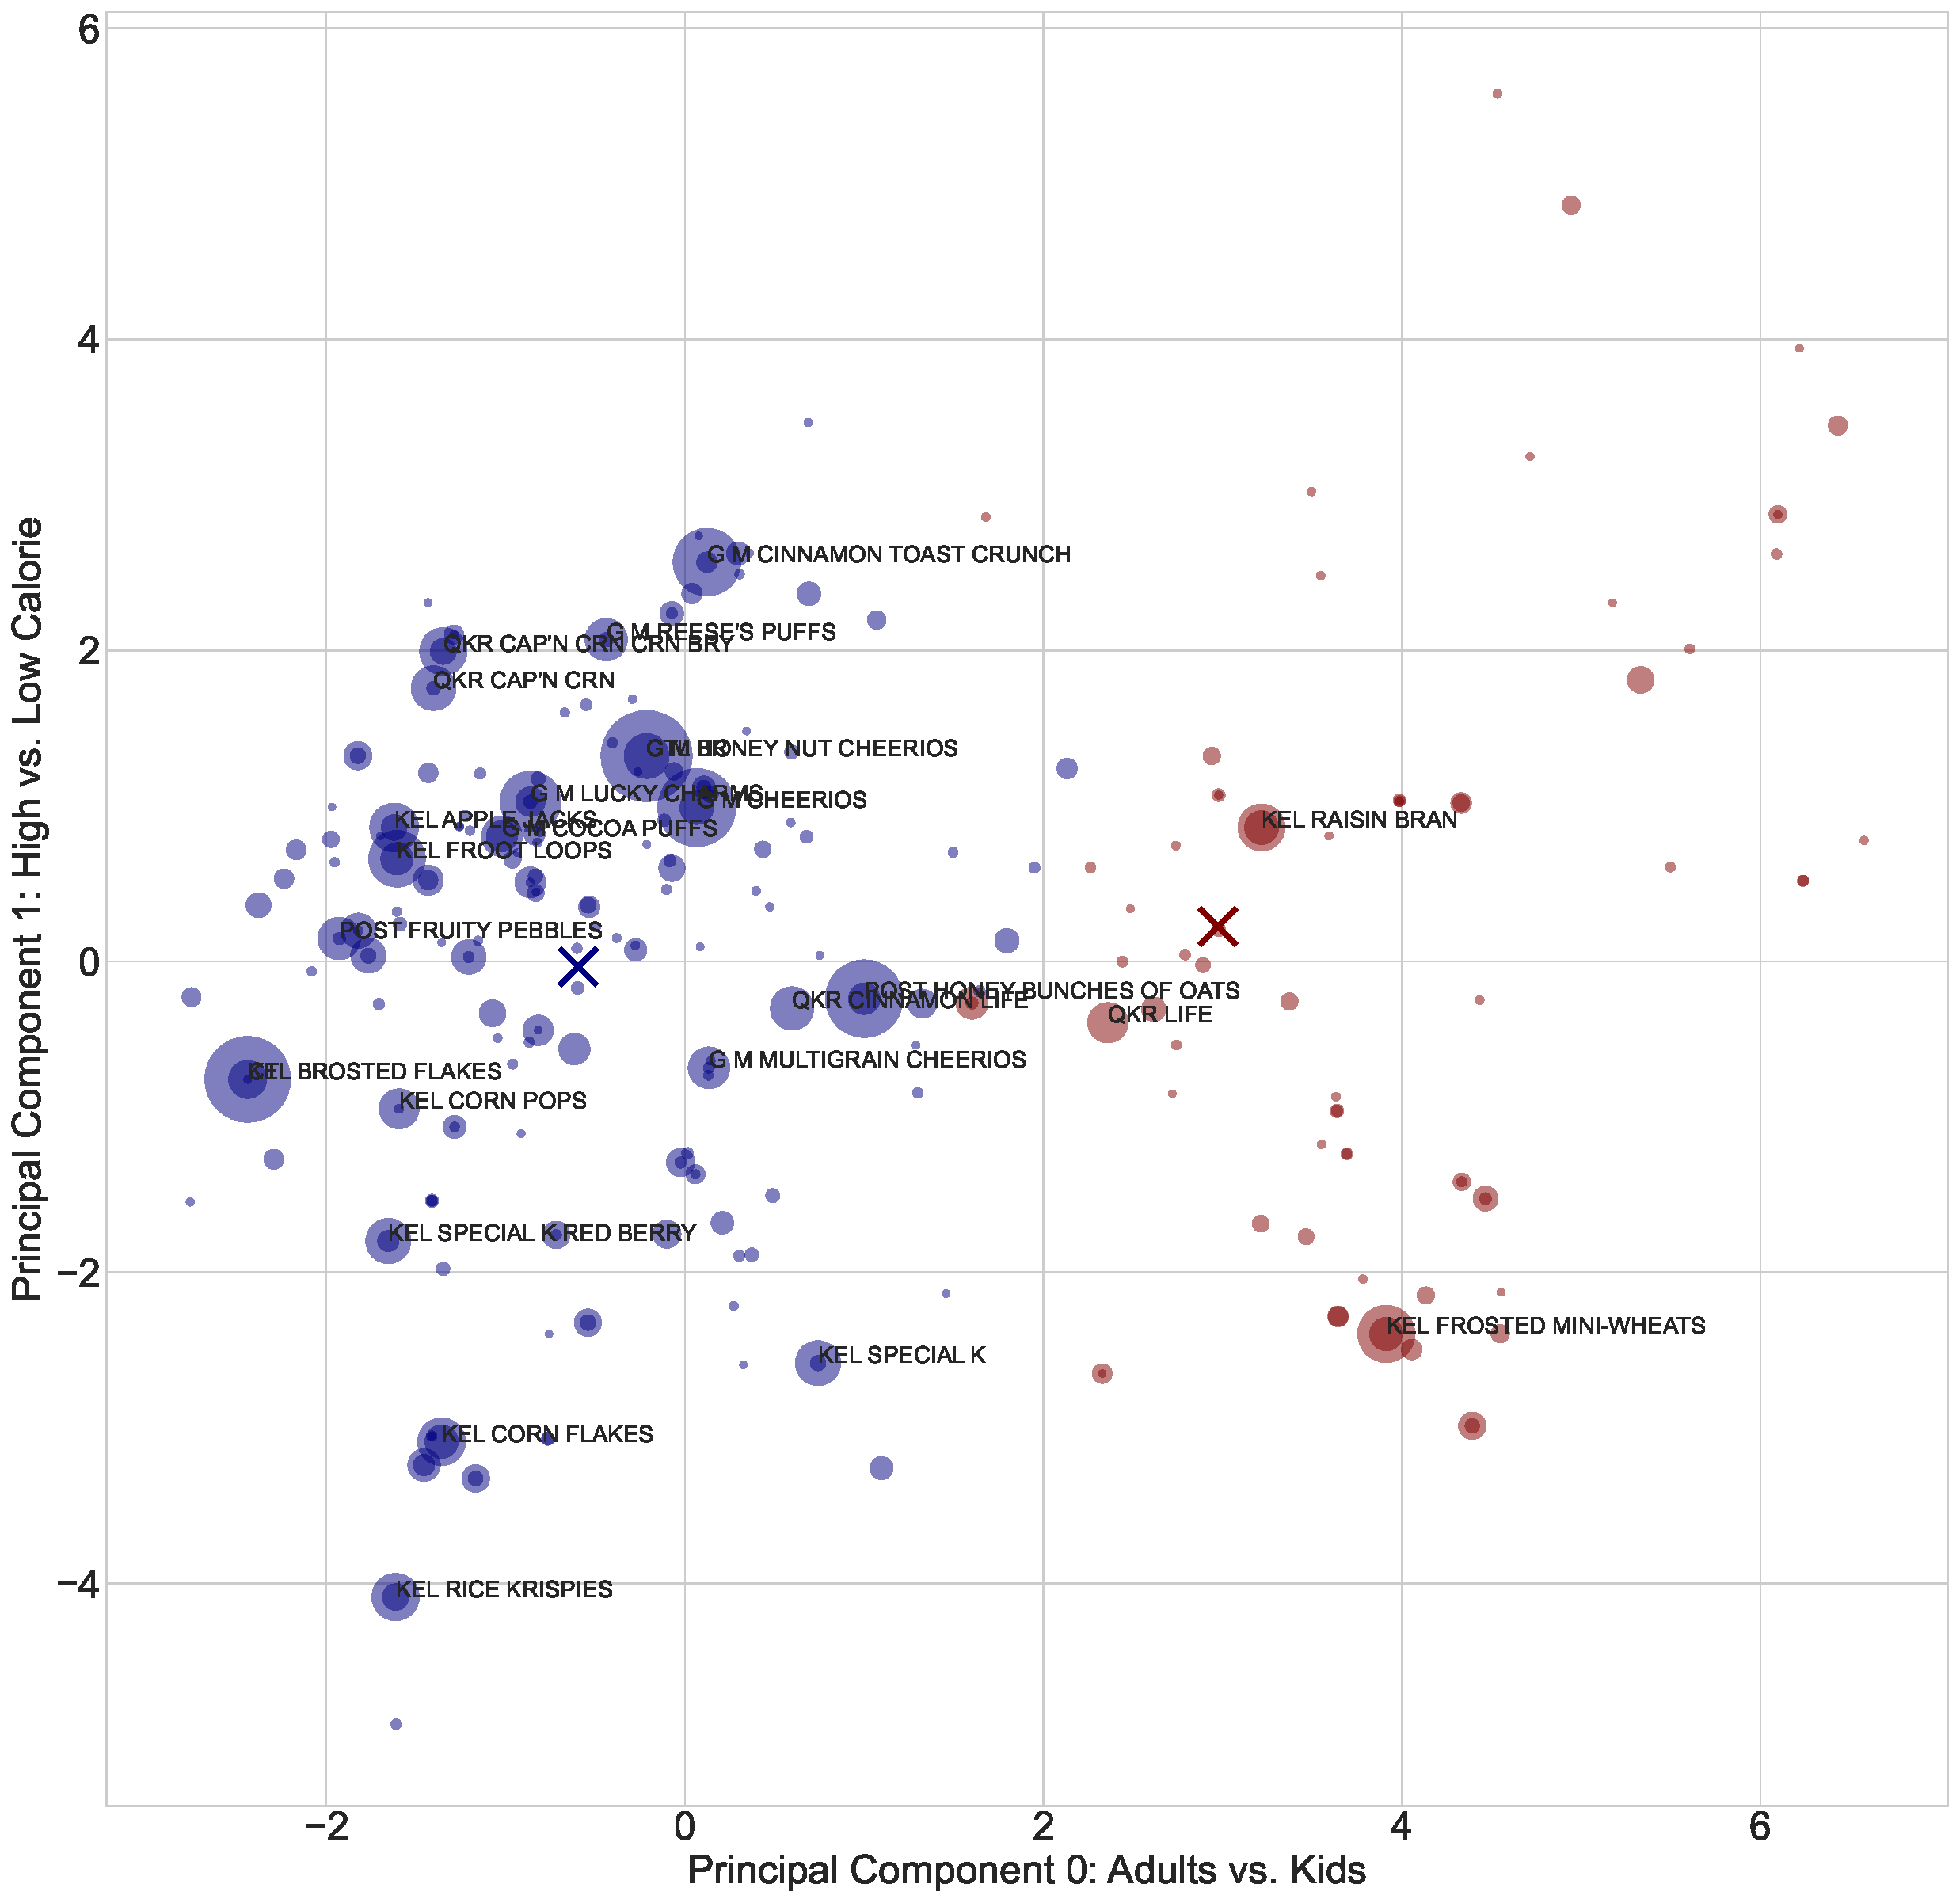
\includegraphics[height = \textheight ]{../common ownership/figures/pca_nests.pdf}
\end{center}
\end{frame}



\begin{frame}[plain,label=maindemand]{Demand Estimation}
\begin{itemize}
\item We estimate demand system using \texttt{PyBLP} (Conlon Gortmaker RJE 2020)
\item Highlights:
\begin{itemize}
\item We estimate market size from milk and egg purchases.
\item Observable demographic preference shocks (income and children).
\item Random coefficients on: (constant, price, branded, servings per box, 3 PC's)
\end{itemize}
\item Moments:
\begin{itemize}
\item Own input costs and local demographic variables.
\item ``Local'' Gandhi-Houde differentiation instruments
\item We convert these into 21 ``optimal instruments"
\item 520 micro-moments to get $\Pi$ and $\Sigma$.
\end{itemize}
\end{itemize}
\end{frame}


\begin{frame}{Implementation: Micro Moments}
Also have 520 ``micro-moments'' grouped by \texttt{DMA-Code/Retail Chain}
\begin{align*}
\mathbb{E} \left[x_{jt} \times y_{it} \mid \text{purchase } \right] 
- \mathbb{E}\left[x_{jt} \times y_{it}  \times \frac{s_{ijt}(\theta_1,\theta_2)}{1-s_{i0t}(\theta_1,\theta_2)}  \right] = 0.
\end{align*}
\begin{itemize}
\item Match observed interactions of characteristics (constant, price, branded, servings per box, PC) \& demographics from the model and the data.
\item Conditional on purchase.
\item We calculate these from Nielsen Panelist data by \texttt{chain-dma-year}.
\item We carefully track \# of observations to get variance calculations.
\item We bootstrap the covariance from the sample (but not model).
\end{itemize}
See Conlon Gortmaker (Micro 2023) for details.
\end{frame}

\begin{frame}{Parameters}
\begin{columns}
\begin{column}{0.4\textwidth}
\scalebox{0.33}{
\begin{tabular}{ll|c|cc|ccc} 
 \toprule 
 Parameter & Variable & \multicolumn{1}{c}{No $\Pi$ } & \multicolumn{2}{|c|}{No $\Sigma$ } & \multicolumn{3}{c}{Full Model} \\ 
 \midrule 
$\theta_2$ & & $\sigma^2$ & $\pi_{kids}$ & $\pi_{income}$ & $\pi_{kids}$ & $\pi_{income}$ & $\sigma^2$ \\ 
 \cmidrule(lr){1-1}\cmidrule{2-8} 
{} &          Constant &        40.102 &       3.837 &      0.333 &     2.505 &   -1.771 &    7.402 \\
{} &                   &         (1.136) &       (0.106) &      (0.080) &     (0.124) &    (0.076) &    (0.496) \\
{} &             Price &         8.263 &       0.676 &     -0.440 &     0.641 &   -0.715 &    0.415 \\
{} &                   &         (0.535) &       (0.027) &      (0.024) &     (0.034) &    (0.021) &    (0.035) \\
{} & Cov(Const, Price) &        18.203 &             &            &           &          &    1.750 \\
{} &                   &         (0.823) &             &            &           &          &    (0.128) \\
{} &             PCA\_0 &               &       0.061 &     -0.056 &     0.081 &   -0.028 &          \\
{} &                   &               &       (0.009) &      (0.005) &     (0.008) &    (0.005) &          \\
{} &             PCA\_1 &               &       0.084 &      0.011 &     0.077 &    0.007 &          \\
{} &                   &               &       (0.009) &      (0.005) &     (0.008) &    (0.006) &          \\
{} &             PCA\_2 &               &      -0.123 &      0.188 &    -0.090 &    0.074 &          \\
{} &                   &               &       (0.011) &      (0.006) &     (0.009) &    (0.006) &          \\
{} &           Branded &               &       0.043 &      0.158 &     0.807 &    0.582 &          \\
{} &                   &               &       (0.045) &      (0.037) &     (0.041) &    (0.041) &          \\
{} &      Servings/Box &               &      -0.048 &     -0.088 &    -0.036 &   -0.008 &          \\
{} &                   &               &       (0.004) &      (0.004) &     (0.004) &    (0.003) &          \\
\midrule 
 $\theta_1$ & & & & & & & \\ 
 \cmidrule(lr){1-1}\cmidrule{2-8} 
{} &            Price &\multicolumn{1}{c|}{3.143}&\multicolumn{2}{c|}{2.445}&\multicolumn{3}{c}{2.472} \\ 
{} &                  &\multicolumn{1}{c|}{(0.011)}&\multicolumn{2}{c|}{(0.025)}&\multicolumn{3}{c}{(0.027)} \\ 
{} &  Unemp x Branded &\multicolumn{1}{c|}{-0.043}&\multicolumn{2}{c|}{-0.016}&\multicolumn{3}{c}{-0.025} \\ 
{} &                  &\multicolumn{1}{c|}{(0.002)}&\multicolumn{2}{c|}{(0.002)}&\multicolumn{3}{c}{(0.002)} \\ 
{} &         Recall 1 &\multicolumn{1}{c|}{-0.259}&\multicolumn{2}{c|}{-0.299}&\multicolumn{3}{c}{-0.344} \\ 
{} &                  &\multicolumn{1}{c|}{(0.083)}&\multicolumn{2}{c|}{(0.073)}&\multicolumn{3}{c}{(0.075)} \\ 
{} &         Recall 2 &\multicolumn{1}{c|}{-0.215}&\multicolumn{2}{c|}{-0.154}&\multicolumn{3}{c}{-0.159} \\ 
{} &                  &\multicolumn{1}{c|}{(0.059)}&\multicolumn{2}{c|}{(0.054)}&\multicolumn{3}{c}{(0.056)} \\ 
{} &         Recall 3 &\multicolumn{1}{c|}{0.035}&\multicolumn{2}{c|}{0.05}&\multicolumn{3}{c}{0.058} \\ 
{} &                  &\multicolumn{1}{c|}{(0.074)}&\multicolumn{2}{c|}{(0.057)}&\multicolumn{3}{c}{(0.062)} \\ 
{} & log(Advertising) &\multicolumn{1}{c|}{0.03}&\multicolumn{2}{c|}{0.03}&\multicolumn{3}{c}{0.03} \\ 
{} &                  &\multicolumn{1}{c|}{(0.002)}&\multicolumn{2}{c|}{(0.002)}&\multicolumn{3}{c}{(0.002)} \\ 
\midrule 
 \multicolumn{2}{l|}{Model Predictions} &  50\% & \multicolumn{2}{c|}{50\%} & 25\% & 50\% & 75\%  \\ 
 \midrule 
 & Own Elasticity           & -2.923 &\multicolumn{2}{c|}{ -2.676 }& -3.055 & -2.812 & -2.592 \\
 & Aggregate Elasticity     & -0.351 &\multicolumn{2}{c|}{ -0.402 }& -0.435 & -0.393 & -0.348 \\
& Outside Good Diversion    &  0.384 &\multicolumn{2}{c|}{  0.570 }&  0.425 &  0.499 &  0.574 \\
\cmidrule{2-8}  
& Lerner (Own Profit Max)   &  0.307 &\multicolumn{2}{c|}{  0.411 }&  0.351 &  0.394 &  0.446 \\
& Lerner (Common Ownership) &  0.351 &\multicolumn{2}{c|}{  0.446 }&  0.372 &  0.428 &  0.501 \\
& Lerner (Big Four)         &  0.444 &\multicolumn{2}{c|}{  0.512 }&  0.408 &  0.497 &  0.621 \\
& Lerner (Monopoly)         &  0.713 &\multicolumn{2}{c|}{  0.648 }&  0.531 &  0.676 &  0.885 \\
\bottomrule 
\end{tabular}
}
\end{column}
\begin{column}{0.6\textwidth}
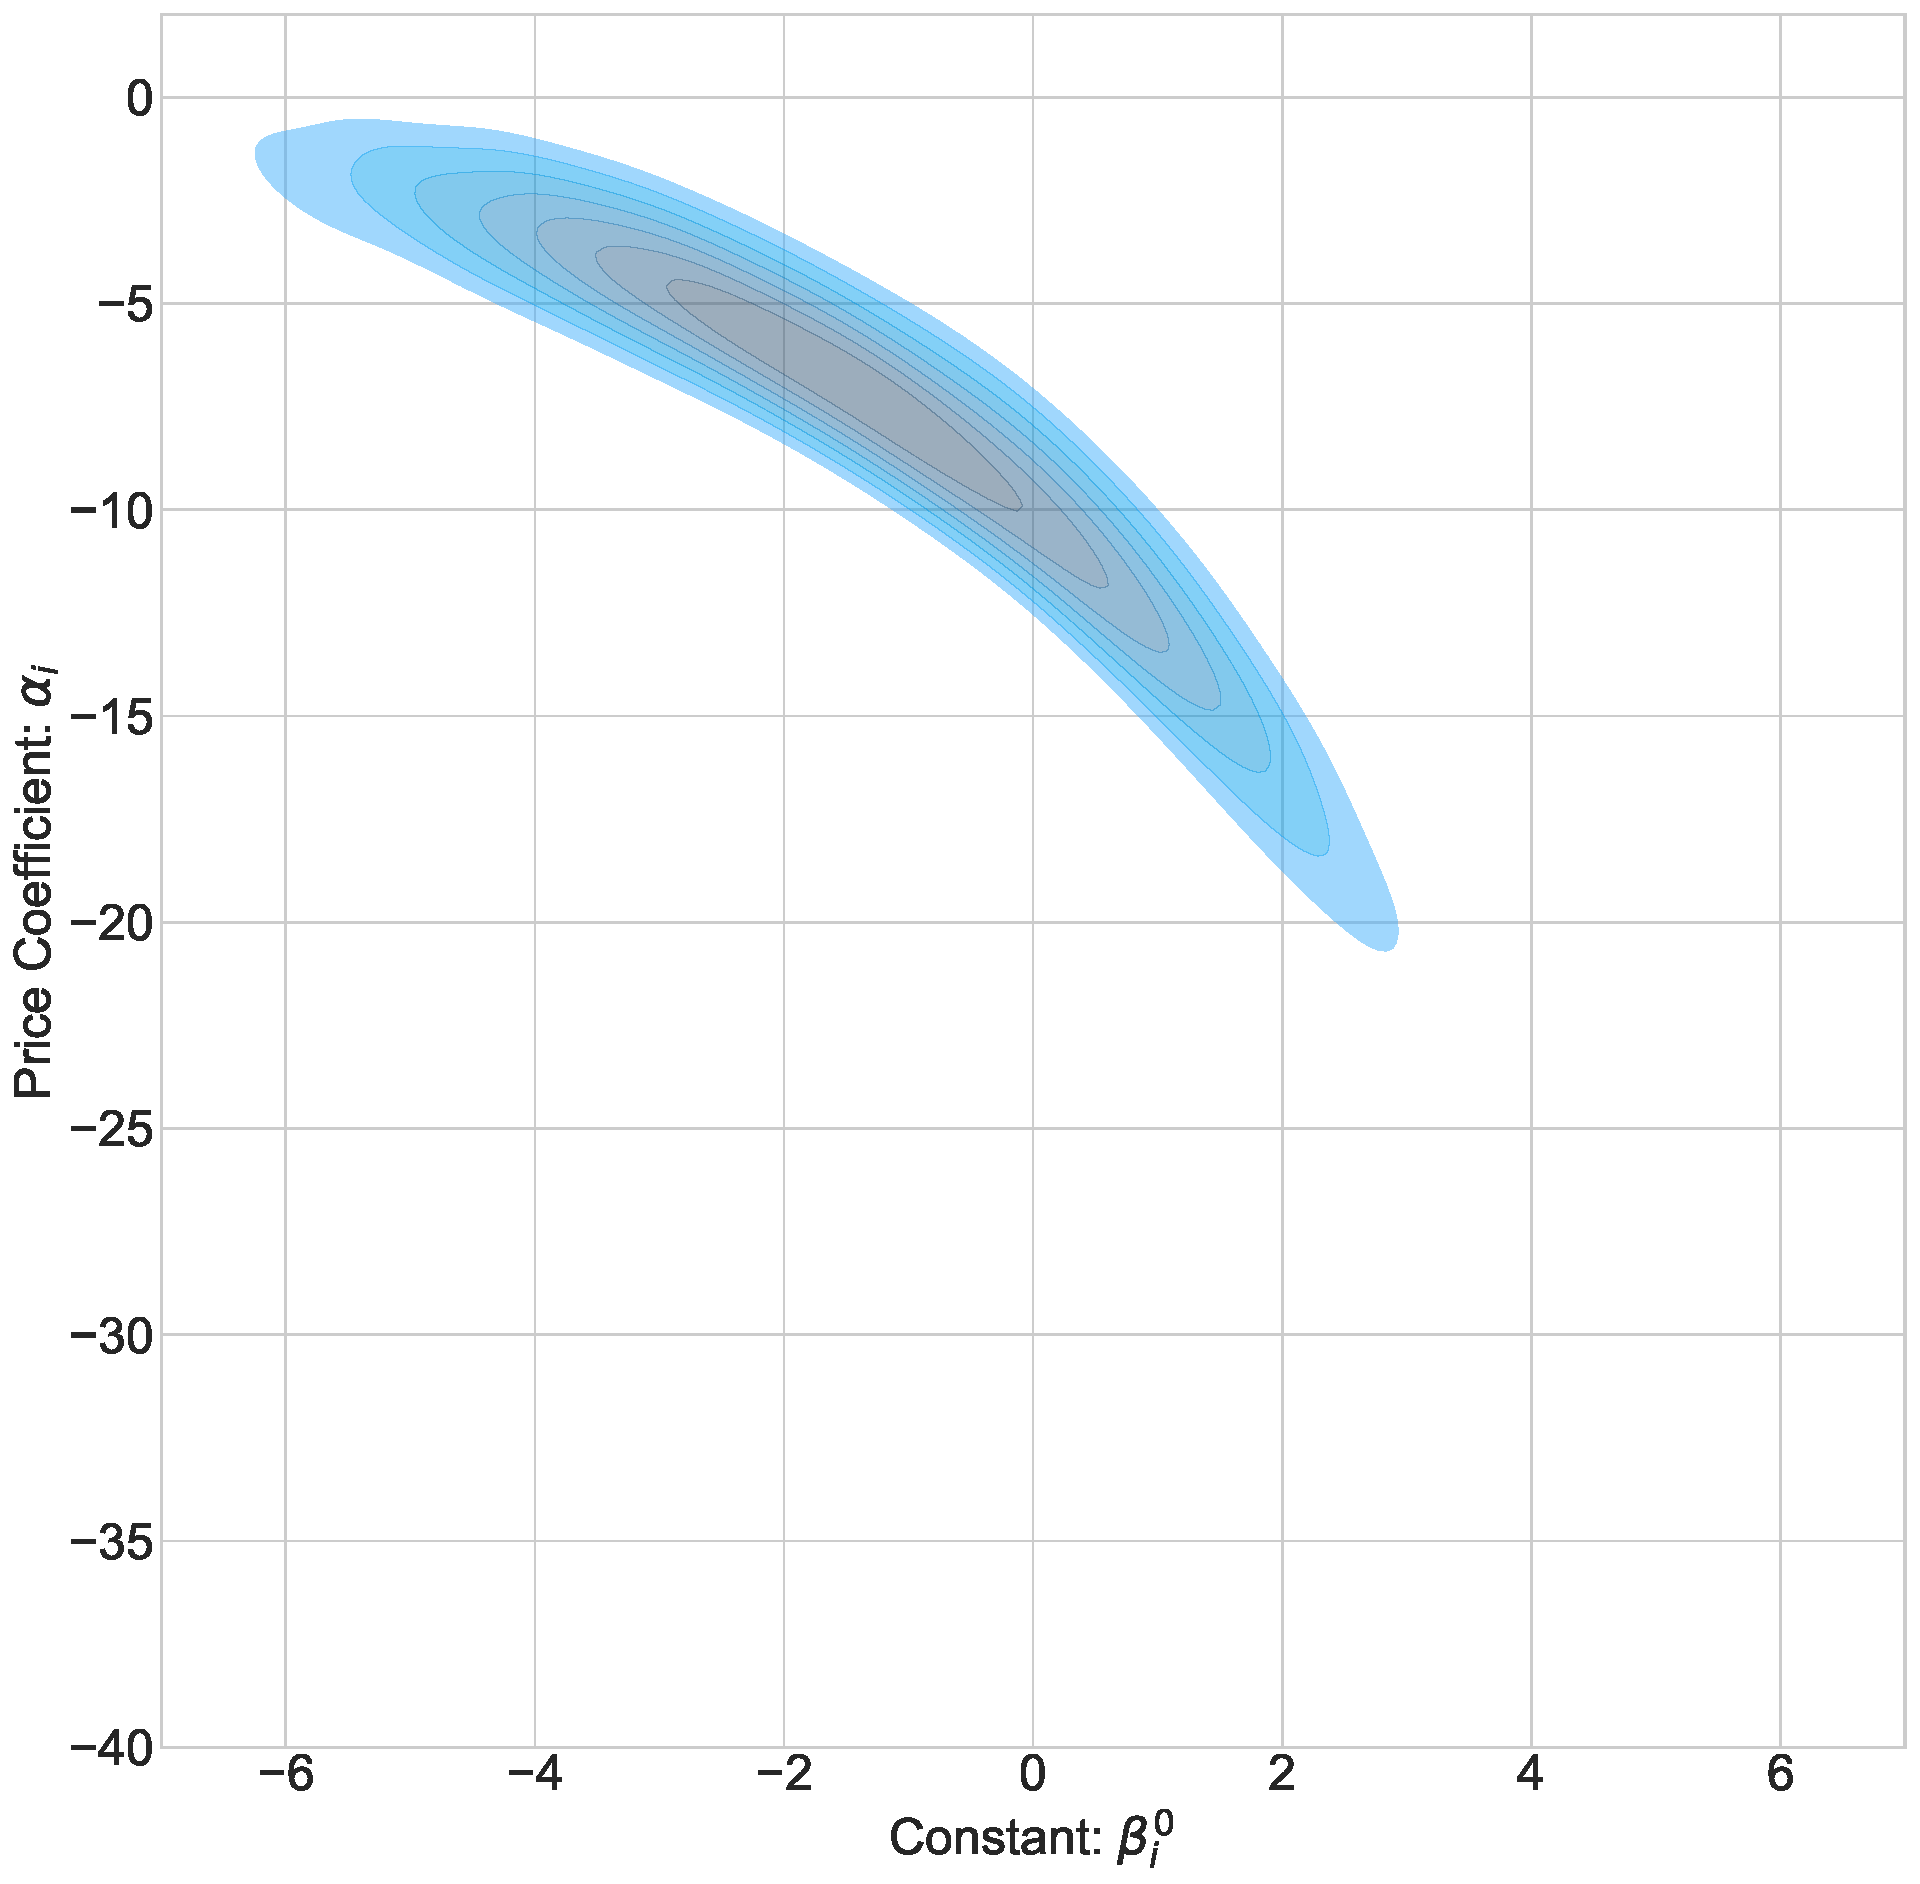
\includegraphics[width=0.9\textwidth]{../common ownership/resources/2d_density_plot.pdf}
\end{column}
\end{columns}
\end{frame}



\begin{frame}{Diversion Ratios}
\begin{align*}
D_{jk} = \frac{\partial q_j}{\partial p_k}/\left|\frac{\partial q_j}{\partial p_j}\right| = \frac{e_{jk}}{e_{jj}} \cdot \frac{q_j}{q_k}
\end{align*}
\begin{itemize}
  \item Easier to interpret than cross elasticity
  \item Higher diversion implies closer competition
  \item See Conlon Mortimer (RJE 2021) for all kinds of tricks.
\end{itemize}
\end{frame}
\begin{frame}[plain]
\begin{center}
\scalebox{0.6}{
\begin{tabular}{lrrrrrrr}
\toprule
{} &  Cheerios &  Special K &  Corn Flakes &  Reese's Puffs &  Capt Crunch &  Froot Loops &  Shares \\
\midrule
HN Cheerios         &      5.07 &       4.27 &         3.75 &           5.33 &         3.58 &         3.48 &    2.69 \\
Frosted Flakes      &      2.46 &       2.54 &         4.54 &           4.00 &         5.35 &         7.24 &    2.65 \\
Cheerios            &     - &       5.91 &         3.13 &           3.19 &         1.36 &         1.77 &    2.10 \\
Honey Bunches       &      2.47 &       2.51 &         2.21 &           2.08 &         1.94 &         1.99 &    1.47 \\
Cinn Toast Crunch   &      3.43 &       2.10 &         1.69 &           3.00 &         1.78 &         1.84 &    1.43 \\
Froot Loops         &      1.26 &       1.19 &         1.64 &           1.69 &         1.82 &        - &    1.18 \\
Lucky Charms        &      2.18 &       1.64 &         1.57 &           2.99 &         1.59 &         1.58 &    1.14 \\
Frosted Mini-Wheats &      0.36 &       0.50 &         0.74 &           0.68 &         0.87 &         1.27 &    1.01 \\
Corn Flakes         &      2.01 &       2.18 &        - &           1.31 &         1.24 &         1.52 &    0.98 \\
Rice Krispies       &      1.50 &       1.72 &         1.56 &           0.89 &         0.68 &         1.25 &    0.96 \\
Apple Jacks         &      0.91 &       0.80 &         1.24 &           1.27 &         1.42 &         2.45 &    0.85 \\
Raisin Bran (KEL)   &      0.46 &       0.47 &         0.63 &           0.78 &         0.82 &         1.24 &    0.79 \\
Special K Red Berry &      0.96 &       1.45 &         0.95 &           0.78 &         0.68 &         0.90 &    0.75 \\
Special K           &      2.06 &      - &         1.18 &           0.71 &         0.44 &         0.58 &    0.74 \\
MG Cheerios         &      1.11 &       0.99 &         0.75 &           0.89 &         0.54 &         0.66 &    0.71 \\
Reese's Puffs       &      1.36 &       0.86 &         0.87 &          - &         1.08 &         1.01 &    0.69 \\
Life                &      1.15 &       1.12 &         1.05 &           1.02 &         1.72 &         0.89 &    0.68 \\
Cocoa Puffs         &      1.18 &       0.92 &         0.95 &           1.47 &         1.05 &         0.97 &    0.67 \\
Capt Crunch         &      0.63 &       0.58 &         0.88 &           1.21 &        - &         1.19 &    0.62 \\
Capt Crunch Berry   &      0.68 &       0.61 &         0.83 &           1.15 &         3.29 &         1.00 &    0.58 \\
Corn Pops           &      0.43 &       0.43 &         0.71 &           0.66 &         0.75 &         1.45 &    0.56 \\
Cinn Life           &      0.76 &       0.75 &         0.83 &           0.84 &         1.59 &         0.78 &    0.54 \\
Fruity Pebbles      &      0.61 &       0.59 &         0.71 &           0.71 &         0.75 &         0.77 &    0.44 \\
\midrule
Own Elas            &      -2.46&       -2.66 &       -2.64 &           -2.70 &        -2.68 &       -2.71 &  - \\
\bottomrule
\end{tabular}
}
\end{center}
\end{frame}


\begin{frame}[plain]{Single Product: Implied Marginal Costs}
\begin{center}
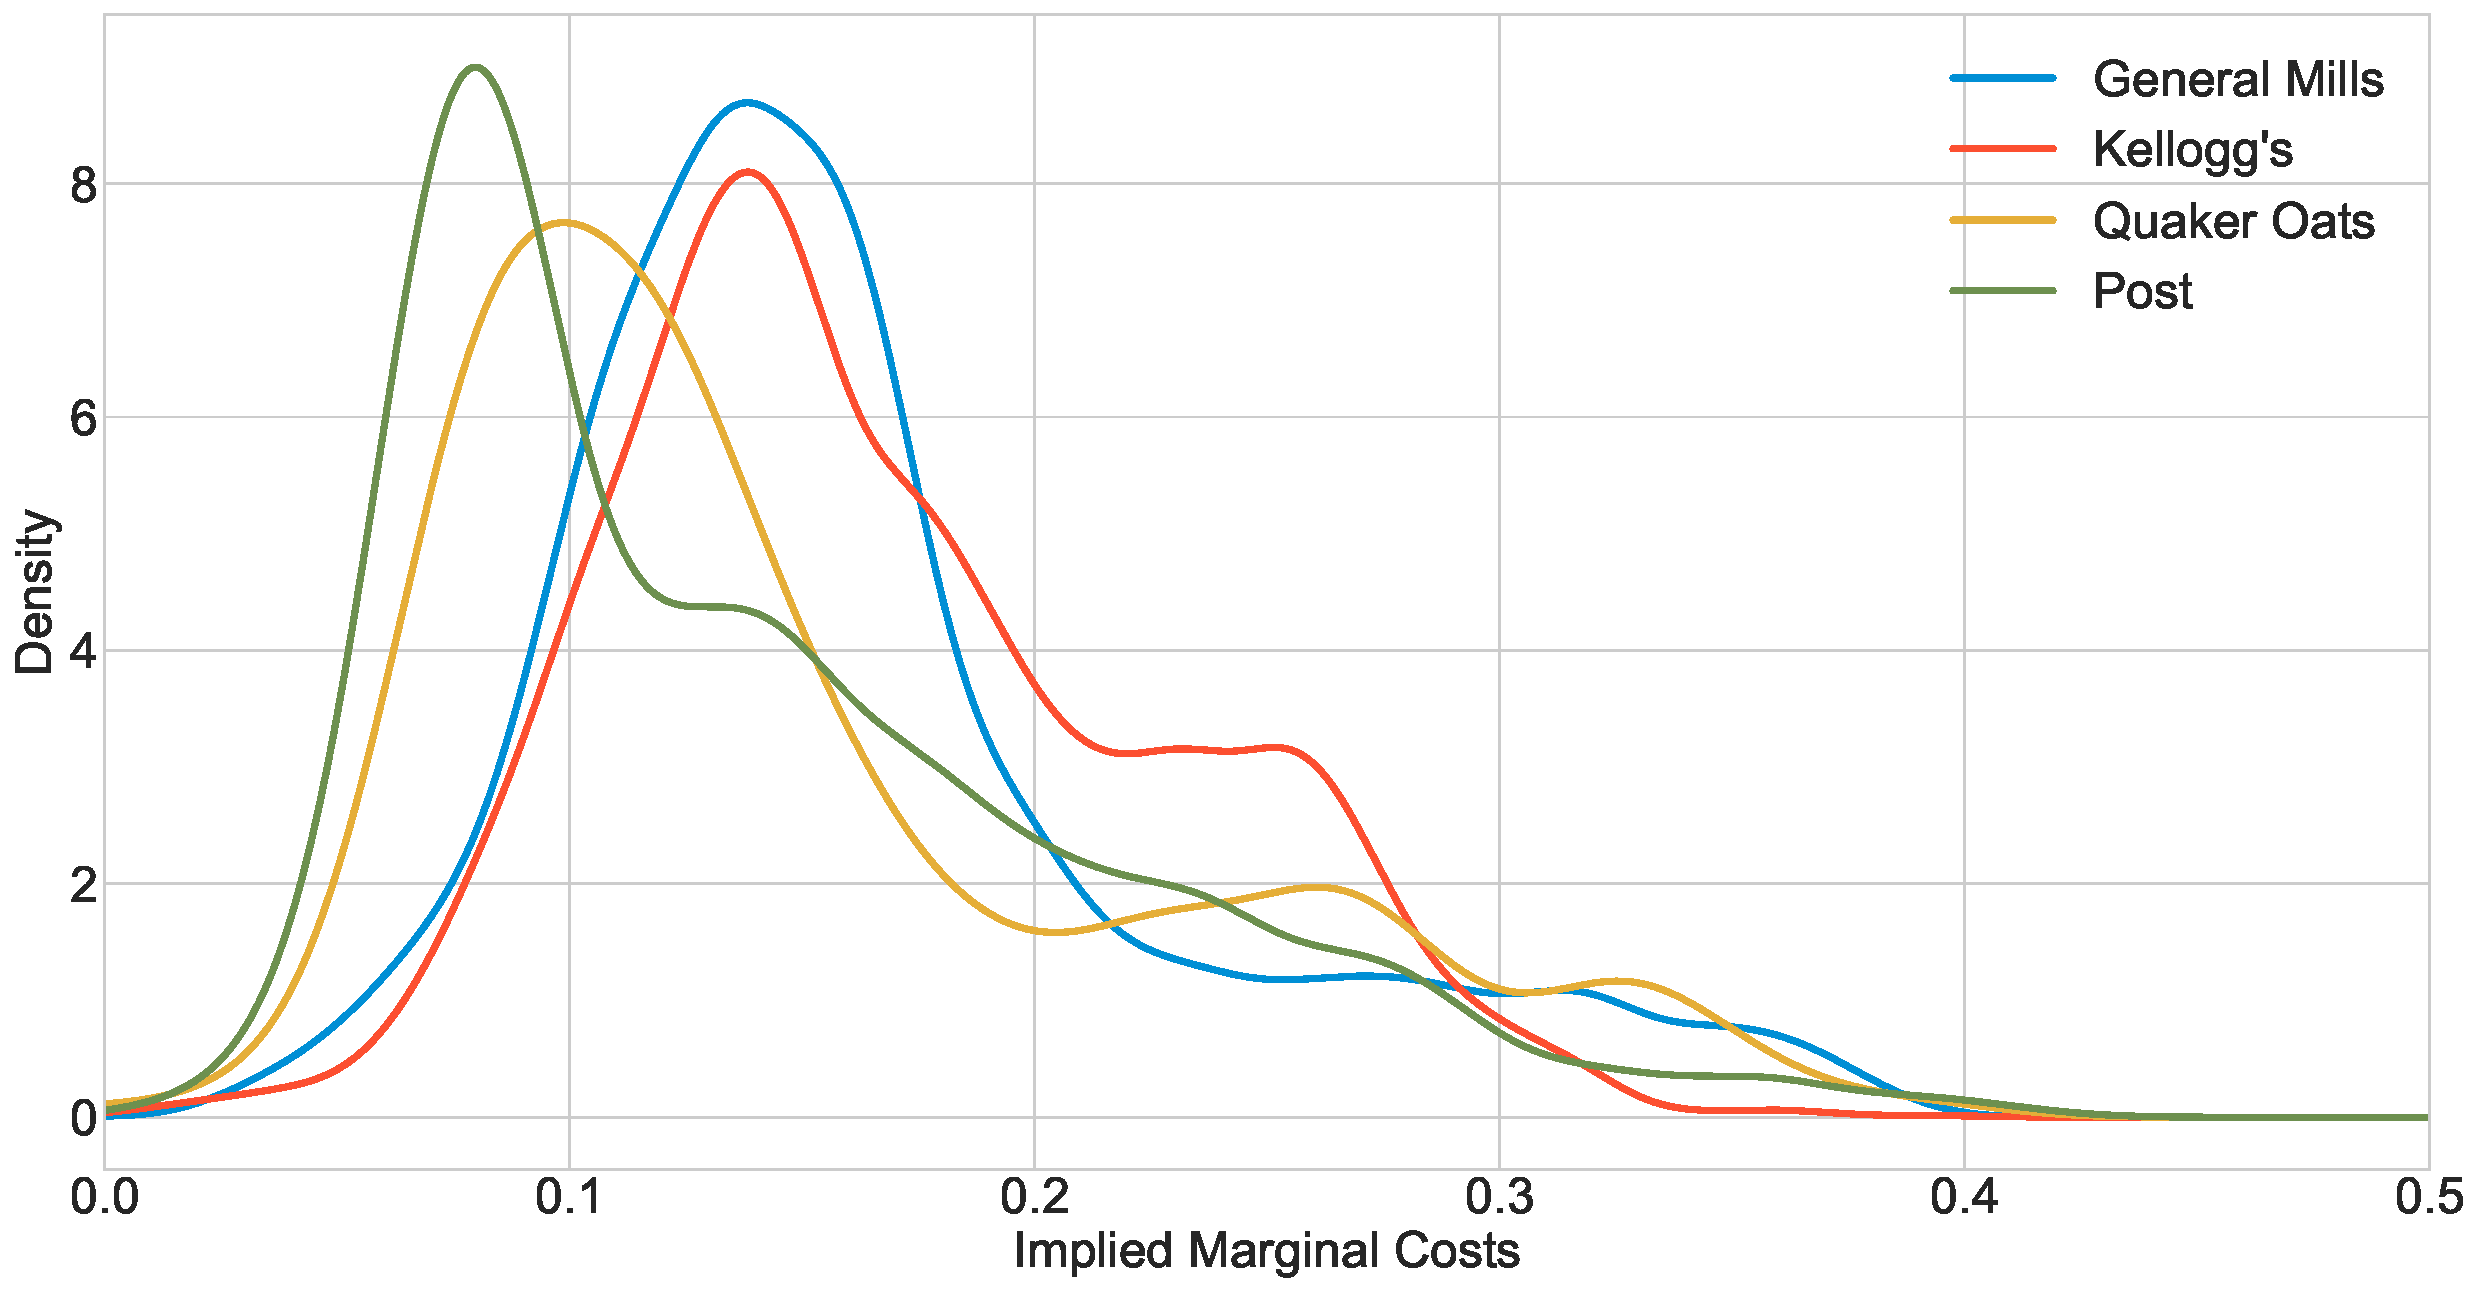
\includegraphics[height =0.8\textheight]{../common ownership/figures/mu_all_bertrand_real.pdf}
\end{center}
\end{frame}



\begin{frame}[plain]{Predicted Markups (Q4 2016)}
\begin{center}
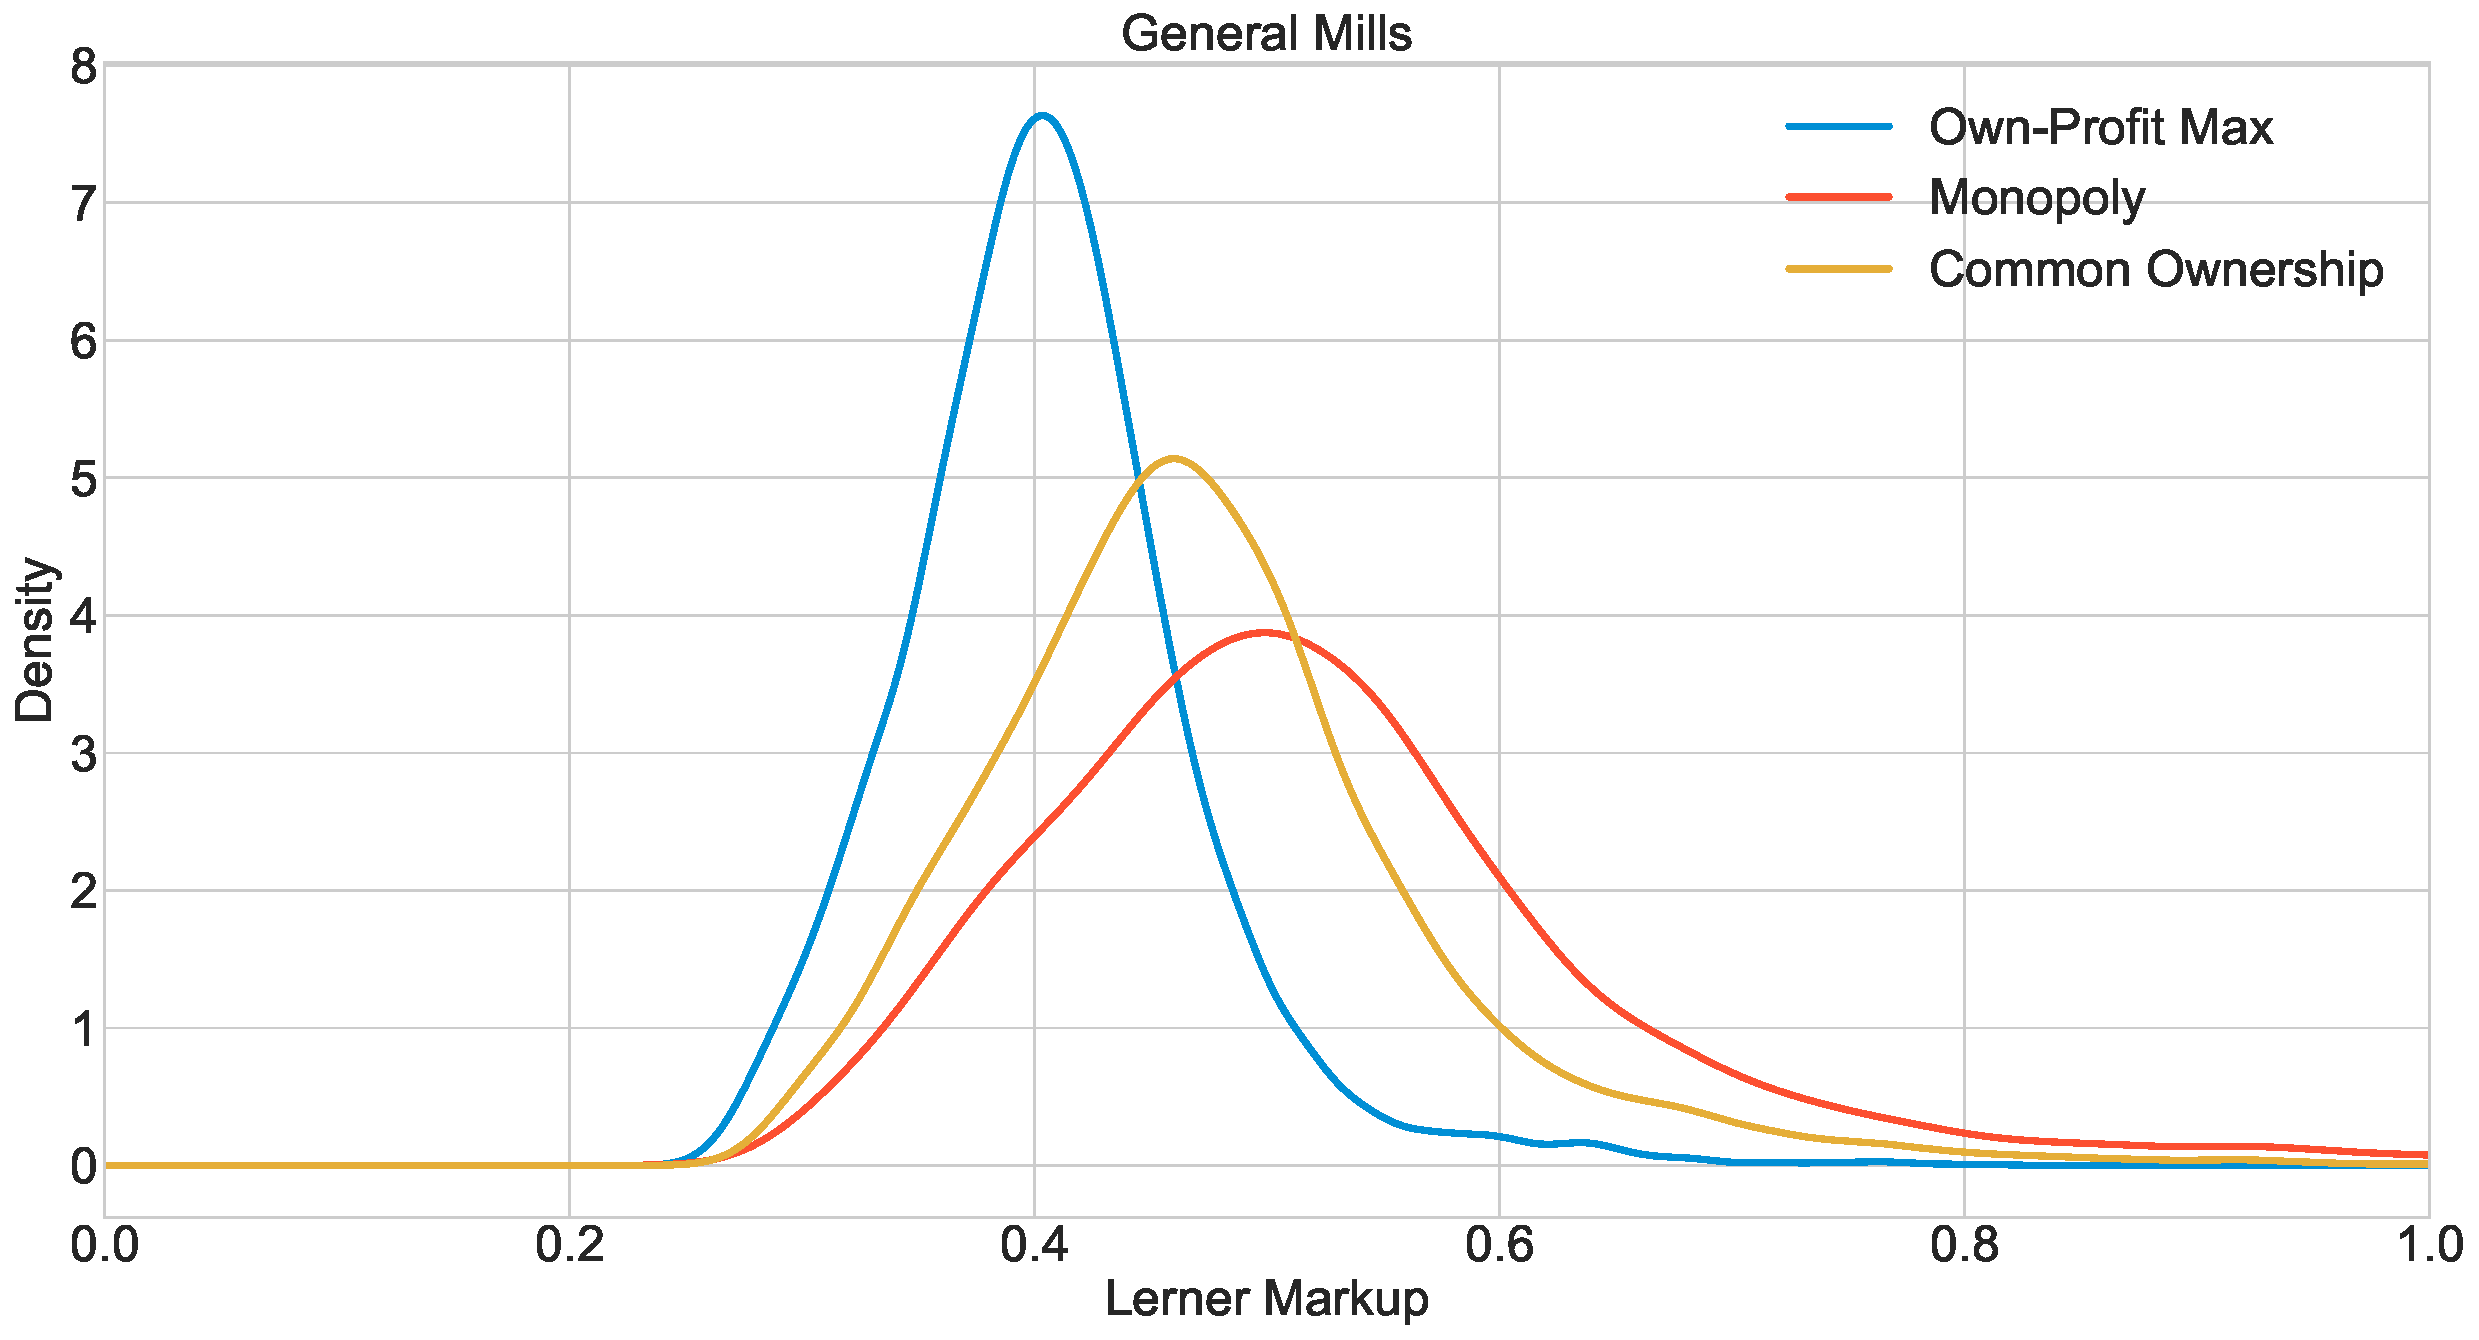
\includegraphics[width = 6.5cm]{../common ownership/figures/mu_gm_real.pdf}
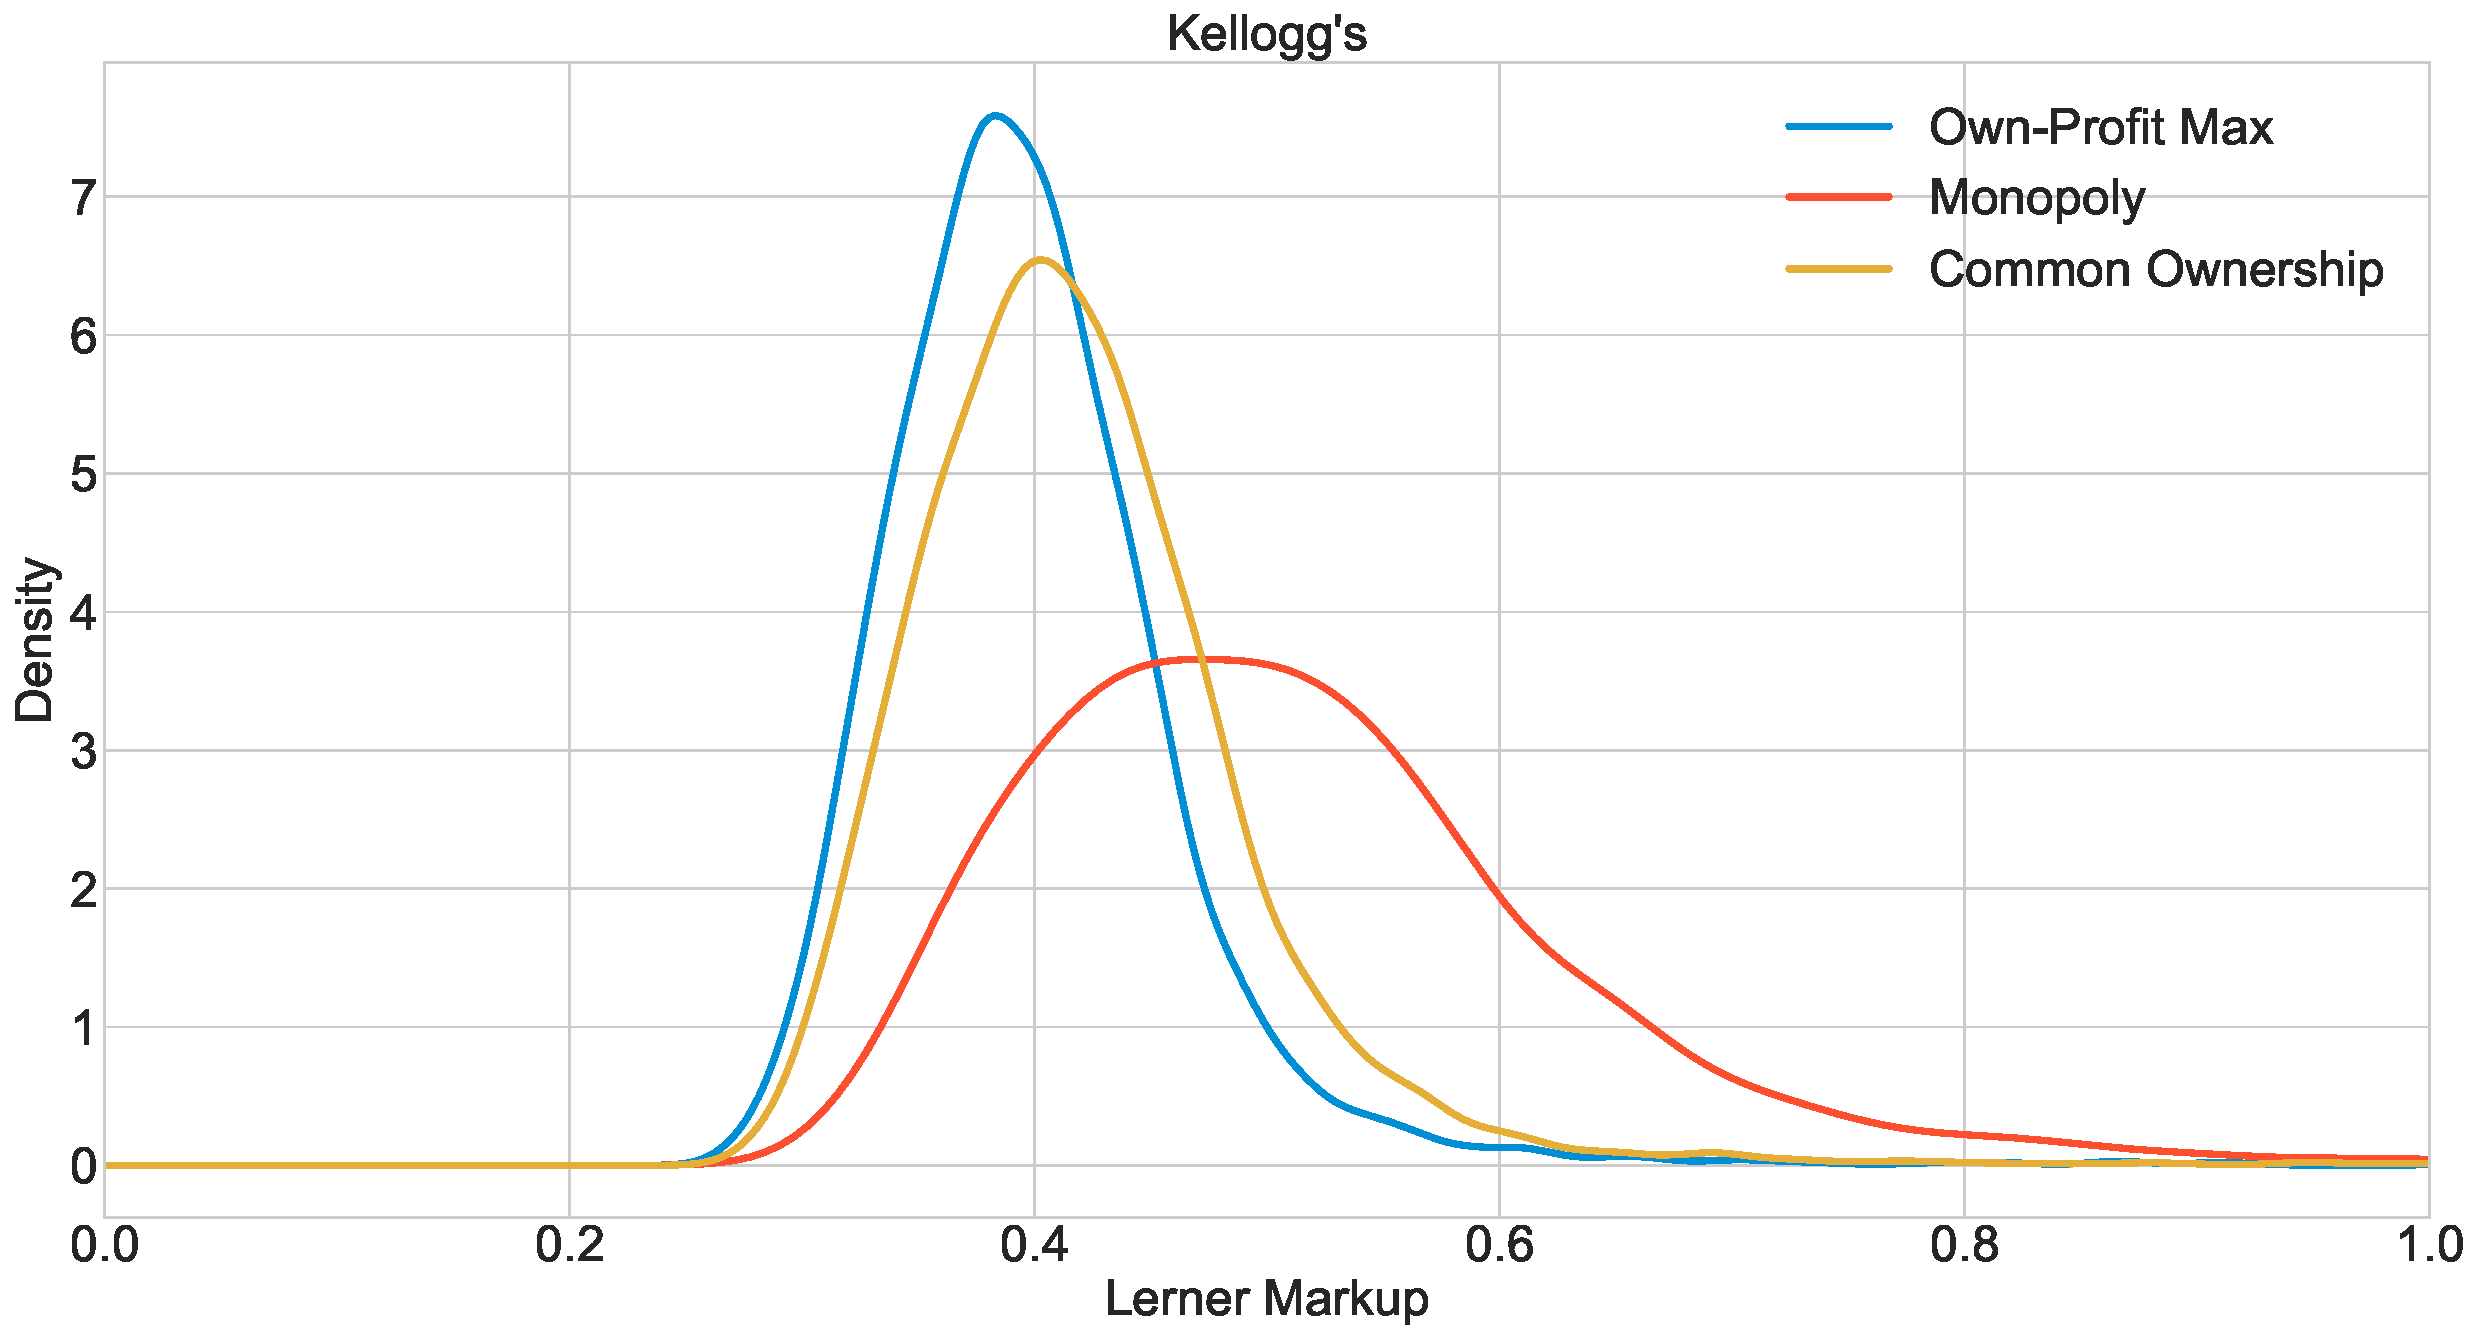
\includegraphics[width = 6.5cm]{../common ownership/figures/mu_kel_real.pdf}\\
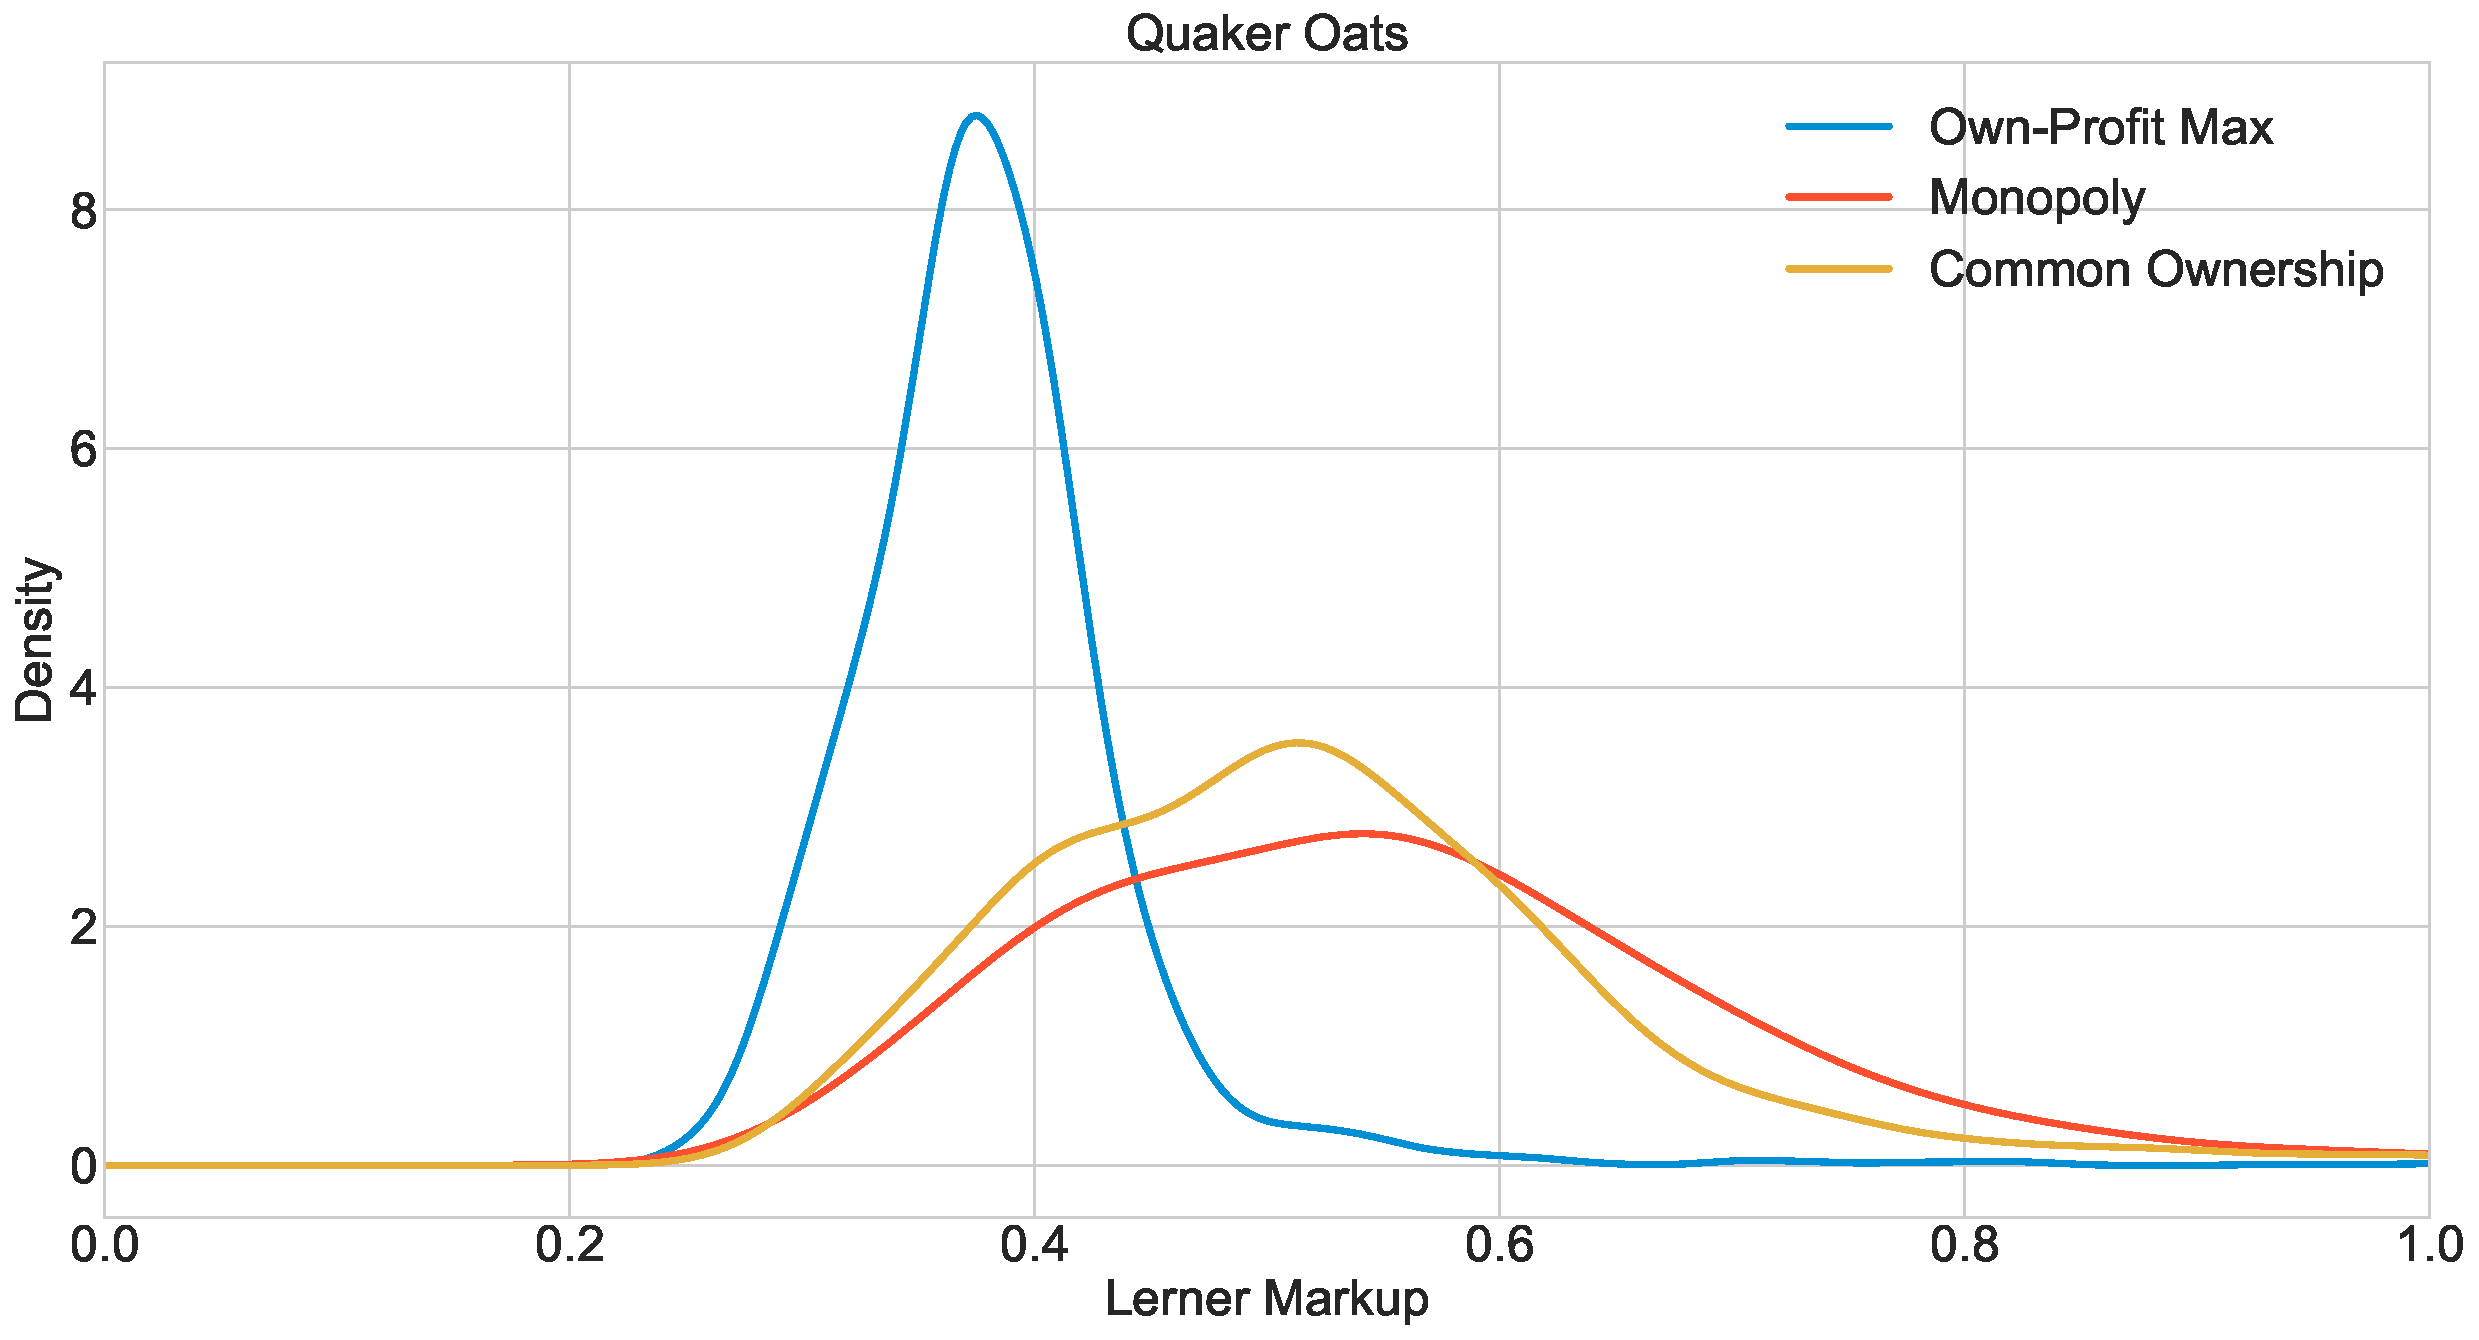
\includegraphics[width = 6.5cm]{../common ownership/figures/mu_qkr_real.pdf}
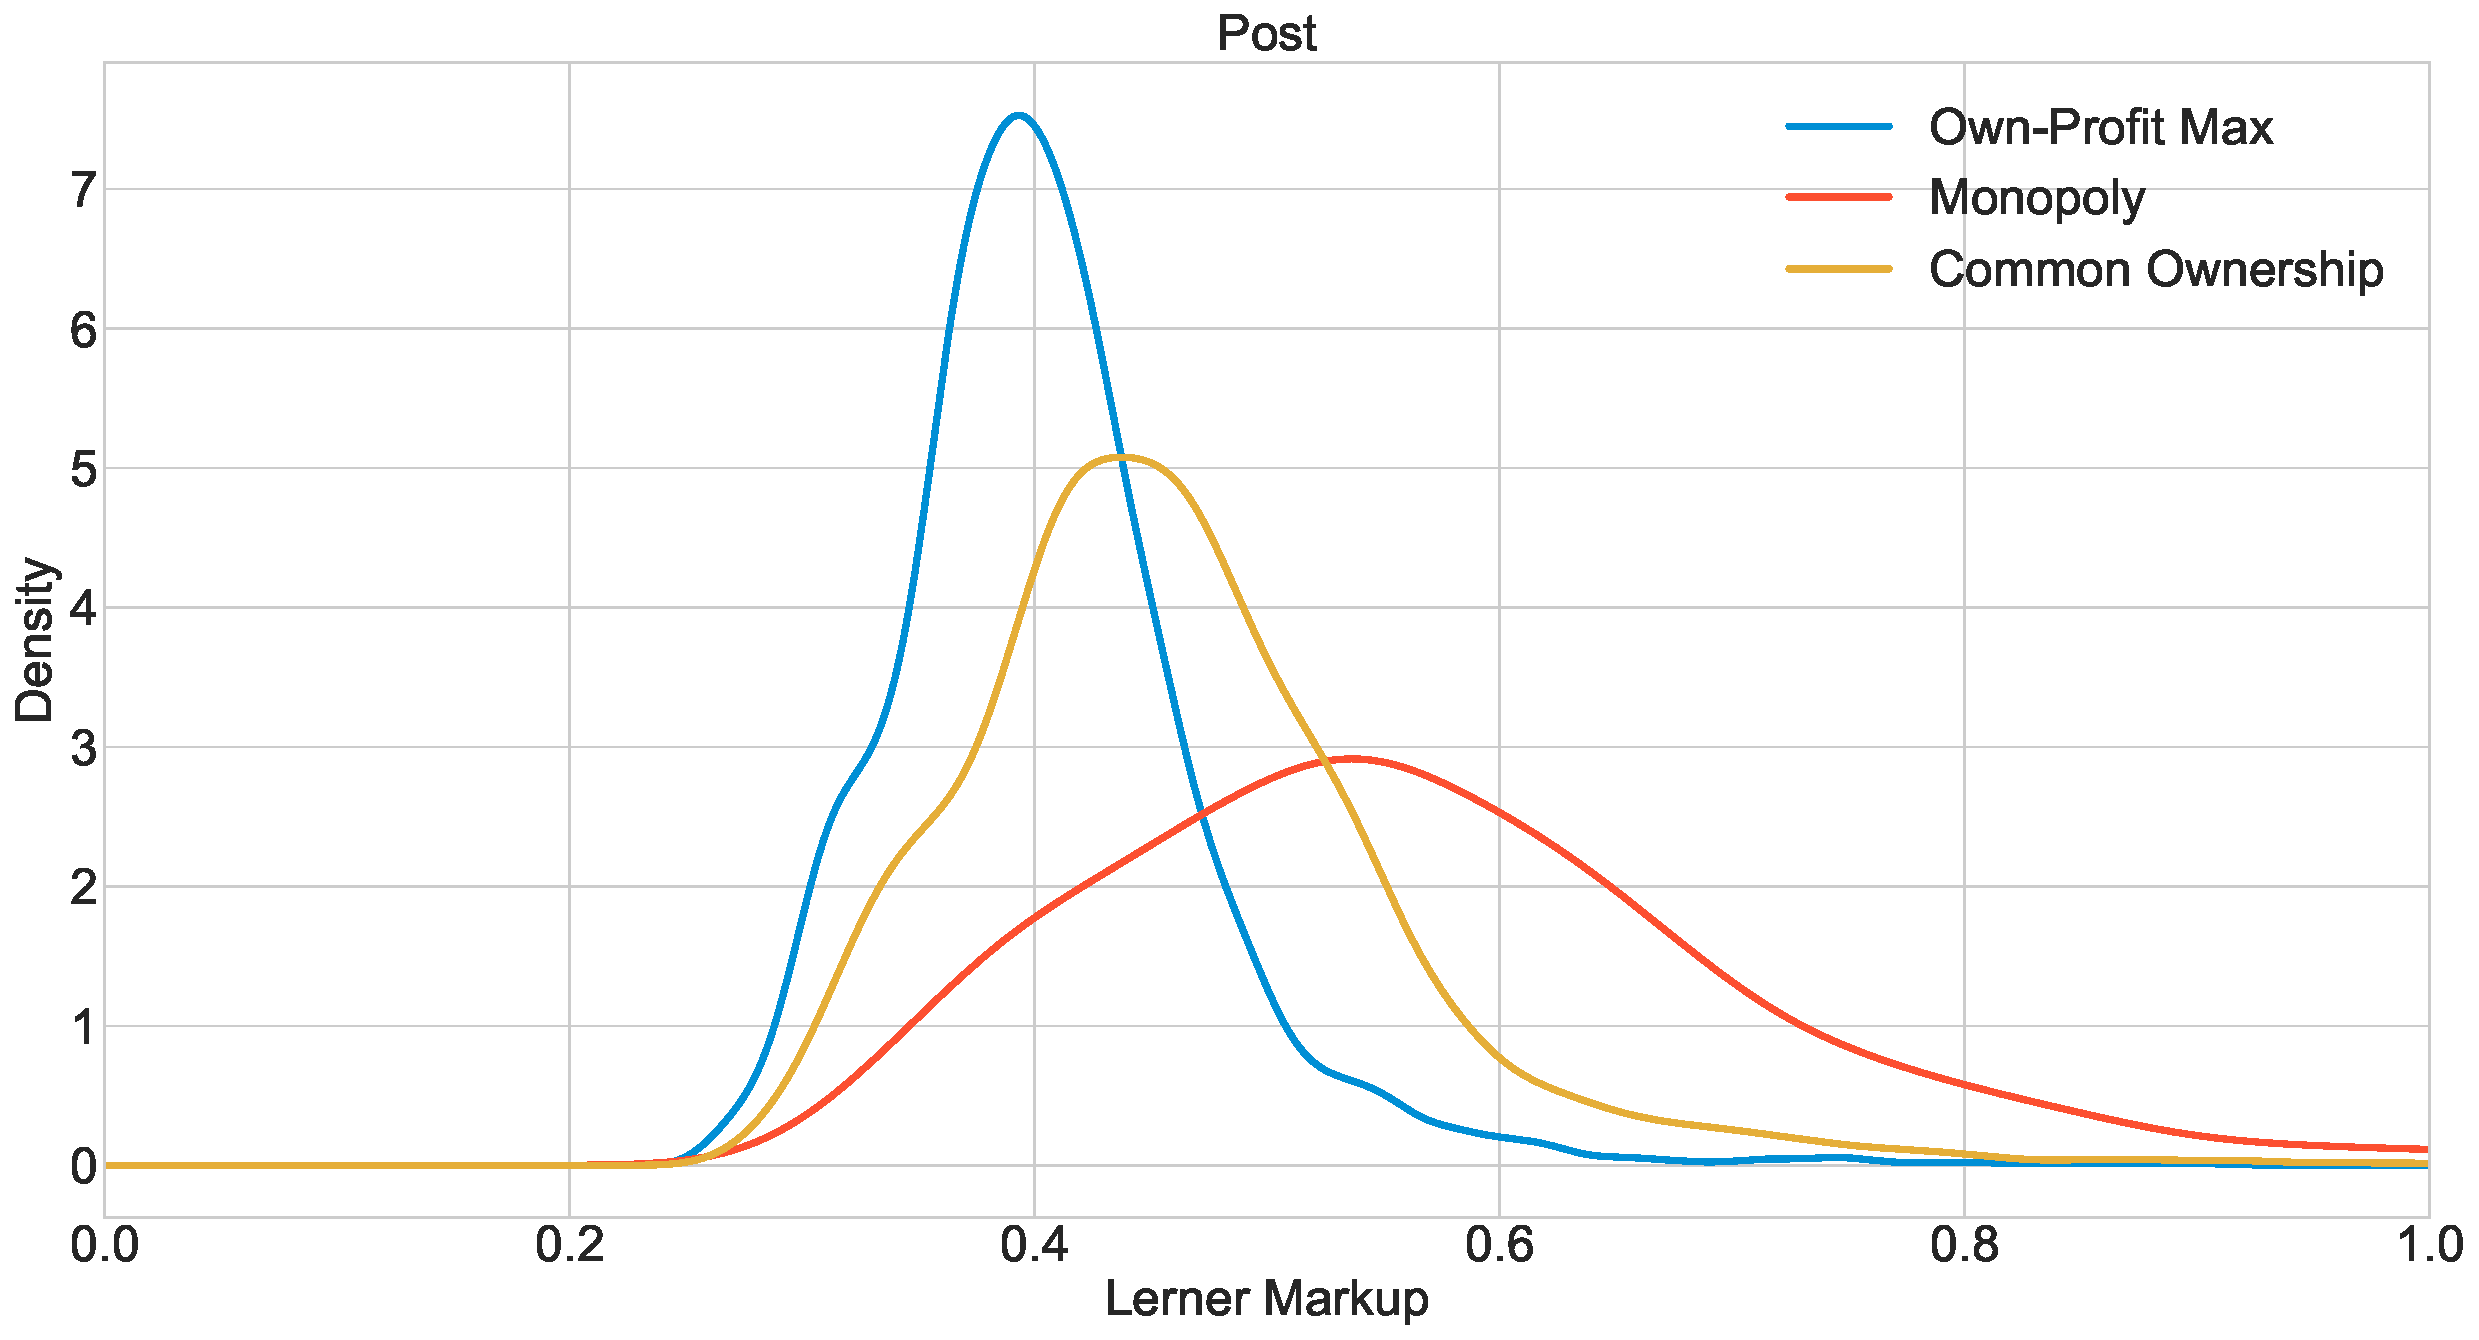
\includegraphics[width = 6.5cm]{../common ownership/figures/mu_post_real.pdf}
\end{center}
\end{frame}


\begin{frame}[plain, label=merger]{Counterfactual Price Increases}
\begin{center}
\scalebox{0.75}{
\begin{tabular}{lrrrrrrrr}
\toprule
{} &  GM-KEL &  GM-QKR &  GM-POST &  KEL-QKR &  KEL-POST &  QKR-POST &  Monopoly &  $\kappa^{CO}$ \\
\midrule
GIS     &    6.94 &    1.53 &     3.30 &    -0.03 &     -0.09 &     -0.05 &     12.22 &           4.81 \\
K       &    6.69 &   -0.03 &    -0.06 &     1.46 &      3.43 &     -0.03 &     12.07 &           6.87 \\
PEP     &   -0.21 &    8.86 &    -0.22 &     8.72 &     -0.22 &      4.48 &     22.41 &          10.67 \\
POST    &   -0.10 &   -0.08 &     7.43 &    -0.09 &      7.98 &      1.75 &     17.49 &           8.49 \\
Overall &    4.49 &    1.10 &     2.25 &     1.08 &      2.40 &      0.57 &     12.50 &           6.01 \\
\bottomrule
\end{tabular}

}
\end{center}
\vspace{1cm}
NB: Computed using marginal costs as predicted by own-profit maximization.\\
Greater than pairwise mergers, 48\% of way to monopoly.\\
Private label provides a LOT of discipline.\\
Strategic substitutes: Negative correlation of $(\beta_{i0}, \alpha_{i})$
\end{frame}

\appendix

\begin{frame}[plain,allowframebreaks,noframenumbering]{References}
    \bibliography{references}
\end{frame}


\end{document}